\chapter{Legal and Ethical Challenges of Decentralised Data Environments}
\label{chap:legal}

\begin{tcolorbox}[colback=royallavender!40]
The content of this Chapter has already been partially included in the articles published during this Thesis \citep{esteves_fostering_2022,asgarinia_who_2023,florea_is_2023}.
\end{tcolorbox}

This Chapter discusses the legal and ethical challenges of the impact of data-driven innovation in society, in particular, related to the emergence of PIMS as a service that helps individuals have more control over the processing of their data.
While some studies have recently been published on the intersection of Solid and data protection requirements, as reviewed in Section~\ref{sec:sota_solid_data_protection}, plenty still has to be overcome to have a `legally-aligned' personal datastore.
This interdisciplinary discussion relies on the collaborations fostered through the PROTECT project, and other EU-funded projects described in Section~\ref{sec:projects}, as well as through the participation in the W3C DPVCG work with data protection law experts.

Section~\ref{sec:motivation_legal} describes the emergence of decentralised personal information management systems as a way to give users more control over their personal data and the challenges that still need to be overcome in order to have to a GDPR-aligned personal datastore.

Section~\ref{sec:policies_consent} discusses the usage of OAC policies as a precursor of consent for Solid, which can enable compliance with several GDPR requirements including the transparent information obligations of Articles 13 and 14 and the conditions to obtain valid consent pursuant to Articles 7 and 4.11.

Section~\ref{sec:automation_consent} argues whether the automation of consent can be performed while maintaining the `informed', `freely given' `specific' and `unambiguous' character of GDPR consent.
In particular, the specificity of purposes and processing operations and the distinction between data controllers and recipients is further analysed through a `legal+tech' approach, relying on GDPR's requirements and on the OAC and PLASMA implementations. 

\section{The emergence of decentralised PIMS}
\label{sec:motivation_legal}

As previously mentioned in Section \ref{sec:def_data_protection_law}, the governance of data flows, and in particular of \textit{personal} data flows, has been a topic of discussion since the early 1970s and 1980s, when the Fair Information Practice Principles (FIPPs) \citep{cate_failure_2006} and Convention 108 \citep{council_of_europe_convention_1981} were first created, to GDPR and subsequent personal data-related regulations being developed in countries such as Brazil or India \citep{bradford_brussels_2019}.
Most of these instruments rely on the existence of an accountable entity that is responsible for establishing the purpose of processing personal data from a natural person, who has rights that must be respected for said processing to be considered compliant with the law.
This model has been the most prevalent since most personal data are stored in large centralised databases under the control of only a certain number of Big tech companies, however, it does not account for cases where the processing is shared among different entities which have distinct purposes or rely on unsuitable legal bases, or the information overload that prevents individuals from actually understanding what they are consenting to \citep{benshahar_more_2014}.
As such, new data governance systems that assist individuals in having more control over their data and trust in data processing services, such as \textit{data cooperatives}, \textit{data trusts}, \textit{data commons} or \textit{personal data sovereignty} schemes, are being proposed \citep{viljoen_relational_2021,craglia_digitranscope_2021} and are even starting to be regulated, such as the new requirements on data intermediation services described in the DGA \citeyearpar{noauthor_regulation_2022}.

In this context, the emergence of decentralised PIMS for the Web, such as the personal datastores model promoted by Solid and studied in this Thesis, has earned many advocates in the last years.
In particular, when it comes to trust, the usefulness and ease of use of digital personal datastores have been proven to be an important factor in increasing citizens' trust in personal data-handling services by allowing them to share their sensitive data for the `public good' while maintaining a sense of control over their data \citep{mariani_explaining_2021}.
Moreover, while these decentralised solutions are not without their faults, as has been shown by blockchain-related scandals in the financial services industry \citep{zetzsche_ico_2019}, their Semantic Web-based counterparts have been gaining a large number of adopters recently as such systems can actually allow its users to choose who can access their data and, therefore, actually shift the power balance in favour of the individuals.
By detaching the storage of data from the data processing services and promoting the usage of Web standards, individuals can move their data between storage providers, use the same data across different services and choose which services and applications best suit their preferences and needs without being locked out of the access to their data \citep{verbrugge_towards_2021,ilves_roadmap_2019}.
This user-managed access to data represents a considerable change from the current \textit{status quo}, where individuals must usually accept an application's privacy policy in order to use it, while personal datastores present the next step towards having an actual negotiation of privacy terms between individuals and data processing entities.
Such systems are also promoted by the EDPS as a mechanism to enable personal data sovereignty where ``Individuals, service providers and applications would need to authenticate to access a personal storage centre'' in an interoperable manner \citep{european_data_protection_supervisor_techdispatch_2021}.
Additionally, the European data spaces initiative launched by the European Commission \citep{european_commission_communication_2020} follows the same spirit by encouraging the development of infrastructures for data holders and data users to share and reuse data across different services while respecting European data protection law.

While personal datastores' developers have as their main banner that data subjects are `controllers' of their data, this view is incompatible with most data protection-related regulations as \textit{``most [...] legal systems are structured around the identification of an accountable entity''} \citep{chomczyk_penedo_selfsovereign_2021} which is given duties in order to ensure that their data processing activities do not affect data subjects' fundamental rights.
In addition, personal data processing activities often involve a complex web of parties that share control of the usage, storage and collection of data for distinct and shared purposes, a fact that makes the compliance with the information requirements described in GDPR's Articles 12 to 14 quite challenging and difficult to implement \citep{lovato_more_2023} -- compliance with such requirements is usually dealt with by providing lengthy and complex notices which are not easy to understand and place a significant burden on data subjects as they have to deal with at least one notice for personal data processing service they use \citep{terpstra_improving_2019,linden_privacy_2020}.
Although these notices usually address the information required by the law, in no way do they fulfil the `informed' character of consent, as prescribed in GDPR's Article 4.11, as it is impossible for data subjects to understand the plethora of terms and conditions of all the personal data handling services that are used nowadays, from smartphone applications to personalised streaming of content, and to give consent in a freely, specific, informed and unambiguous way \citep{mohan_analyzing_2019}.
Beyond consent management, notices are also an inefficient way for data subjects to exercise their rights.

As such, recently, there has been legal work in identifying the different roles and responsibilities that distinct entities occupy in decentralised systems and how said systems can be used to facilitate the exercise of data subjects' rights, fulfil the data protection principles of privacy by design and by default and improve the clarity and transparency of personal data handling processes in contrast to the existing landscape \citep{janssen_personal_2020}, as described in Section~\ref{sec:sota_solid_data_protection}.
Nevertheless, work still needs to be done to align such decentralised systems with the legal requirements, in particular, related to the identification and enforcement of a lawful basis and transparent purpose that justify the access to data.  
Particularly, in this Thesis, the focus is positioned on how to obtain valid consent in Solid, according to the GDPR, while promoting the usage of automation to improve the current information overload felt by data subjects in terms of consent management.
Accordingly, in this Chapter, the introduction of a semantic policy layer, based on the vocabularies described in Chapter~\ref{chap:vocabularies}, for providing the necessary information to obtain informed and valid GDPR consent is studied from a technical and legal angle.

% FROM THE PAPER: In particular, we focus on the processing of health data (considered a special category of personal data under the GDPR) for biomedical research purposes.}

It is likewise important to distinguish between what can be technologically or legally enforced.
Although technically a certain app or service can be restricted to only access certain data, by being allowed to read data from a personal datastore, it can also copy it, even if within a decentralised setting this is not necessary at all.
Thereupon, the realm of law comes into play.
Although the wishes of the data subjects, as stated by the preferences they have stored in their personal datastore, have a role to play in the negotiation of privacy terms between data subjects and data controllers \citep{verborgh_paradigm_2017}, their legal value is still up to debate, as these are quite new technological tools which are still to be argued and tested in the court of law.
\section{Policies as a precursor of consent}
\label{sec:policies_consent}

This Section discusses the usage of OAC policies as a tool to express consent in advance for Solid and how such policies can enable compliance with several GDPR requirements including the transparent information obligations of Articles 13 and 14.
As such, these policies come as a solution to overcome the shortcomings of Solid's access control mechanism when it comes to dealing with GDPR's information requirements.
Moreover, by enabling the communication of this information, policies can be used as a tool to fulfil the conditions to obtain valid consent under Articles 4.11 and 7 of the GDPR.

\subsection{Distinguishing consent from access control}
\label{sec:distinction}

It is important to make a distinction between the legal notion of giving consent and the technical means used to grant an app, service or user-authorised access to a resource stored in a decentralised personal datastore such as a Solid Pod.

As previously discussed in Section~\ref{sec:sota_solid_access_control}, Solid Pods are decentralised, permission-based data storage environments, by default.
This means that in the absence of a tangible authorisation, resources cannot be accessed by apps or users.
Authorisations can then be provided in a direct and indirect way by accepting requests from apps as they are being received or by setting the rules of access in advance, respectively.

From GDPR's viewpoint, user authorisation is not always required for the processing of personal data, but it also might not be enough for entities to process personal data in a lawful manner in such decentralised settings.
In the first case, it might be \textit{unnecessary} as there are other legal bases in GDPR's Article 6.1 which can be used, beyond consent, that do not involve an active choice being made by the data subject, such as the performance of a contract --Article 6.1(b)-- or the legitimate interests of the data controller --Article 6.1(f)-- \citep{kranenborg_article_2014}.
Taking the former as an example, there is no need to have the consent of the data subjects to access personal data when they have entered into a contract with the data controller and access to said data is necessary for the performance of said contract \citep{european_data_protection_board_guidelines_2019}.
Moreover, if indeed the access is based on the consent of the data subject, then the current status quo of access control in Solid --whether being the WAC or the ACP authorisation mechanisms-- is not enough for obtaining valid consent according to the GDPR, as in Article 4.11 valid consent is described as being a \textit{``freely given, specific, informed and unambiguous indication of the data subject’s wishes''} \citeyearpar{noauthor_regulation_2016}. 

By comparing both the legal and the technical requirements, described in the previous paragraphs, it is possible to arrive at two sets of problematic cases:
\begin{itemize}
    \item[(i)] instances when app providers have a valid legal basis beyond consent to have access to the data, but do not have access to said data as no permission-based authorisation, granted by the data subject, is stored in the Pod; and
    \item[(ii)] instances when app providers use consent as a ground for lawfulness, however, the authorisation available on the Pod does not fulfil the conditions for valid consent according to Articles 4.11 and 7.
\end{itemize}

In this Thesis, the second cluster of cases is explored by discussing whether the introduction of fine-grained access control policies, modelled with OAC, is enough for obtaining valid consent.

\subsection{Introducing OAC policies in the Solid ecosystem} % Introducing OAC policies in the Solid ecosystem: from notice to automated consent
\label{sec:oac_notice_automation}

In addition to a lawful basis for processing, Article 5.1(a) states that personal data should be \textit{``processed [...] in a transparent manner in relation to the data subject''} \citeyearpar{noauthor_regulation_2016}.
The information obligations described in Articles 12 to 14 depict the required information that data subjects must be provided with, regardless of the chosen legal basis, in order to have transparent information regarding the processing of their personal data.
This means that data subjects always have the right to have access to this information, while data controllers are always obliged to provide it, even if the legal basis for processing personal data is not consent.
Additionally, Recital 59 provides that \textit{``Modalities should be provided for facilitating the exercise of the data subject’s rights [...] free of charge [...]''}.
In this context, OAC policies can serve as a modality that enables the data subjects' right to information regarding the processing of their personal data.
In particular, OAC-based agreements stored on Solid Pods, such as the one depicted in Listing~\ref{list:oac_agreement}, resulting from the matching of user offers and data requests, \beatriz{described in detail in Chapter XX, } are thus accessible to data subjects and can be used by them to easily understand whether the specific conditions for accessing data, set on the agreement, vary from their personal preferences stored in the Pod in the form of OAC-based preferences and requirements.

The specific privacy terms that need to be provided by data controllers are specified in GDPR's Articles 13 and 14 and detailed in Table~\ref{tab:GDPR_privacy_terms} as informational items I1 to I19.
As can be checked in Figure~\ref{fig:oac_diagram} and Table~\ref{tab:profile_classes}, the OAC profile provides concepts to express personal data types, legal basis, recipients, purposes for processing, processing operations and the identity of the data controllers accessing the data. 
This leaves out some elements noted in Article 13.1, namely the controller's contact details and its representative, the DPO's contact details, the legitimate interests of the data controller or third party recipient, if the used legal basis is grounded on Article 6.1(f), and information about the transfer of data to third countries or international organisations.
Moreover, Article 13.2, in order to ensure fair and transparent processing, also states that data subjects should be informed about the retention period of the data, the existence of data subject rights, statutory or contractual obligation details if the provision of data is a requirement to enter into a contract or a statutory obligation, including the possible consequences of failing to provide such data, and the existence of automated decision-making.

If the user’s policies do not include all these necessary elements, or if there are discrepancies between them and the data access request, then the data subject should be notified about this information at the time of the data request.
In Solid, as previously stated in Section~\ref{sec:distinction}, access can be granted by (i) accepting requests when starting to use a new application or by (ii) setting the access rules in advance.
In the first case, this is done through an authorisation dialogue, such as the examples provided in Figure~\ref{fig:authorisation-dialogue}, and, in the second, through a Pod management app, such as Inrupt's PodBrowser\footnote{{\url{https://docs.inrupt.com/user-interface/podbrowser/} (accessed on 21 December 2023)}} in Figure~\ref{fig:podbrowser} or Penny\footnote{{\url{https://penny.vincenttunru.com/} (accessed on 21 December 2023)}} in Figure~\ref{fig:penny}.
Figure~\ref{fig:css} illustrates the authorisation dialogue related to the Community Solid Server (CSS)\footnote{{\url{https://communitysolidserver.github.io/CommunitySolidServer/7.x/} (accessed on 21 December 2023)}} and Figure~\ref{fig:ess} the Inrupt's Enterprise Solid Server (ESS)\footnote{{\url{https://www.inrupt.com/products/enterprise-solid-server} (accessed on 21 December 2023)}} Pod and identity providers.
While ESS's dialogue includes some information on the purposes for access and CSS's on the specific types of access being provided, as is visible through the Figures, both dialogues do not include all the elements previously discussed for the user to be able to provide informed consent.

\begin{figure*}[htp]
    \caption[Screenshots of the authorisation dialogues of existing Solid servers (CSS and ESS).]{Screenshot of the authorisation dialogue of the}
    \label{fig:authorisation-dialogue}
    \centering
    \subfigure[Community Solid Server]{
        \fbox{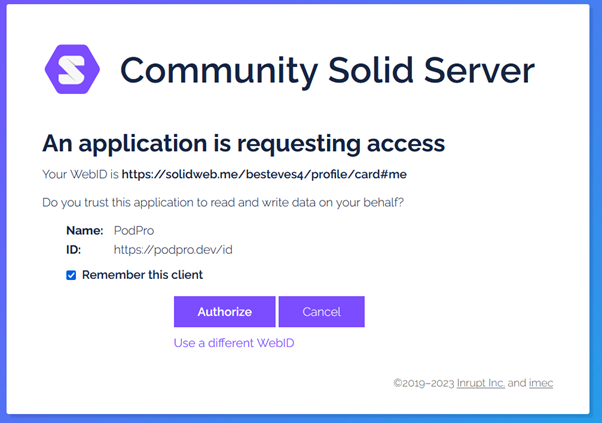
\includegraphics[width=0.4\linewidth]{figures/chapter-5/css.png}}
        \label{fig:css}
    }
    \qquad
    \subfigure[Enterprise Solid Server]{
        \fbox{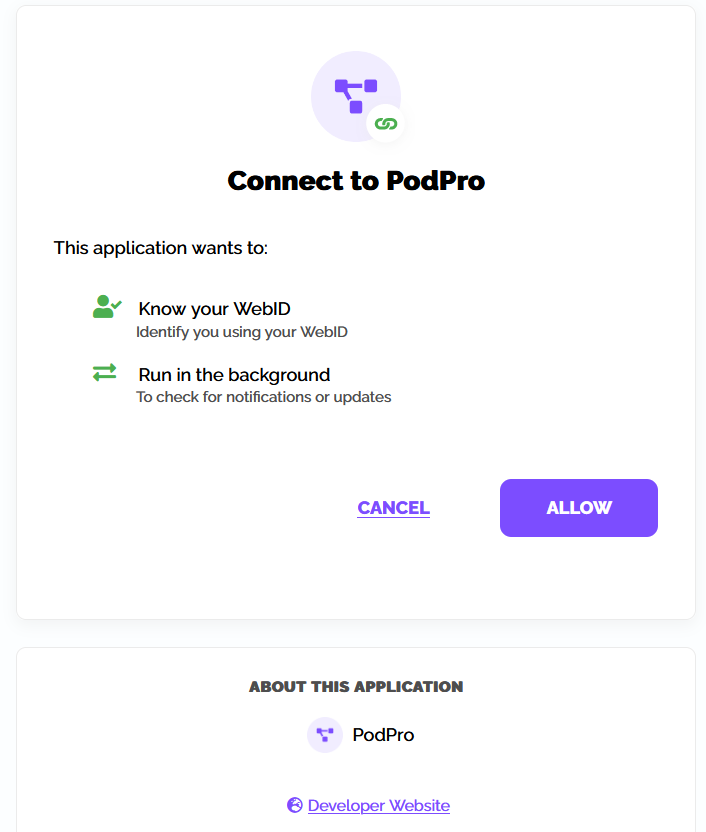
\includegraphics[width=0.4\linewidth]{figures/chapter-5/ess.png}}
        \label{fig:ess}
    }
\end{figure*}

\begin{figure}[htp]
    \centering
    \fbox{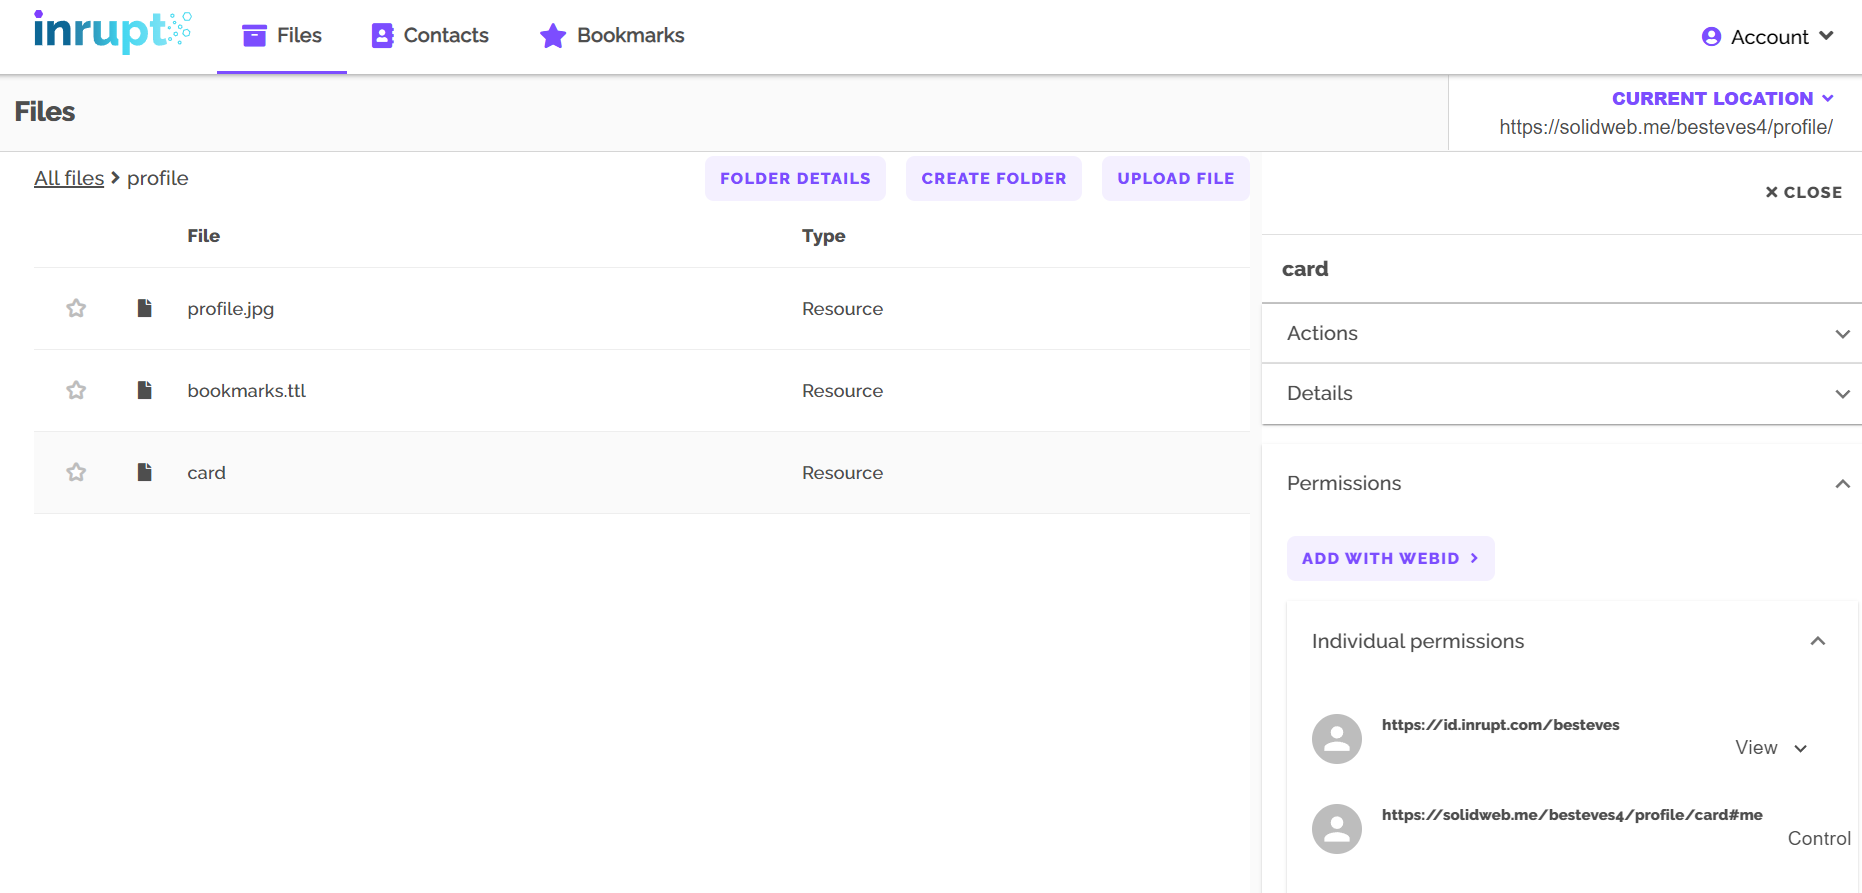
\includegraphics[width=0.9\linewidth]{figures/chapter-5/podbrowser.png}}
    \caption{Screenshot of Inrupt's PodBrowser app to manage data and access grants.}
    \label{fig:podbrowser}
\end{figure}

\begin{figure}[htp]
    \centering
    \fbox{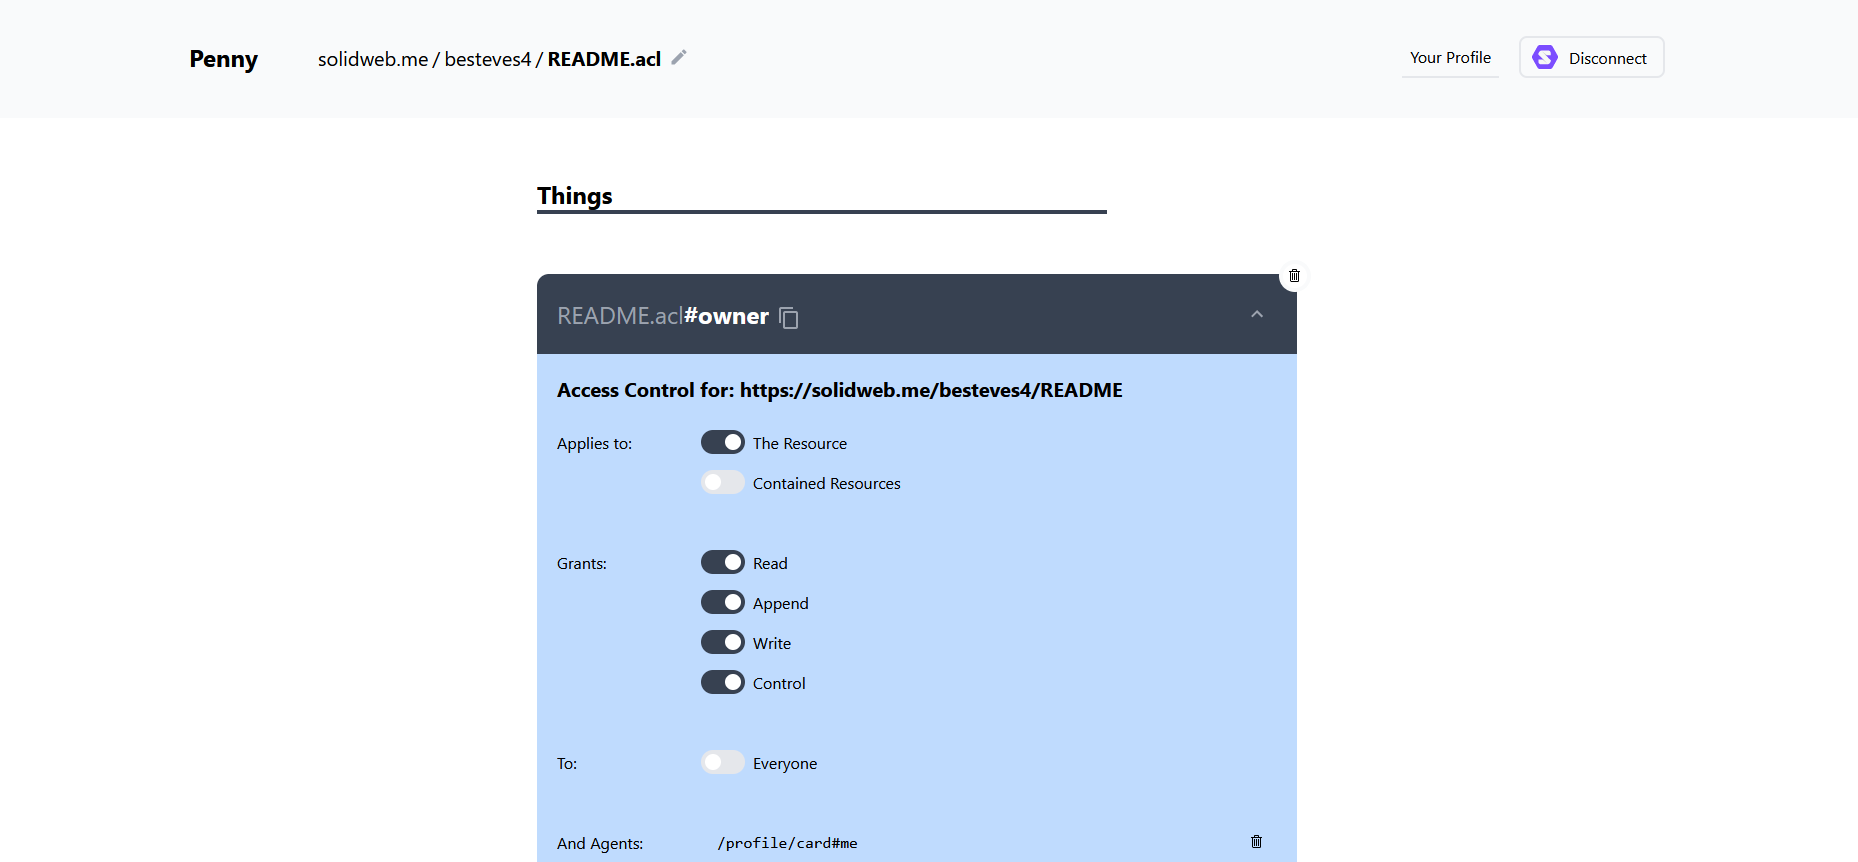
\includegraphics[width=0.9\linewidth]{figures/chapter-5/penny.png}}
    \caption{Screenshot of Penny app to manage data and access grants.}
    \label{fig:penny}
\end{figure}

Furthermore, two more legal challenges should be considered regarding the information obligations set out in the GDPR.
The first relates to how the information is presented to the data subject as GDPR Article 12 states that data controllers have an obligation to provide this information \textit{``in a concise, transparent, intelligible and easily accessible form, using clear and plain language''} \citeyearpar{noauthor_regulation_2016}.
As such, while the user's policies, others' requests and data access agreements can be easily accessed by data subjects if stored in Solid Pods, the implementation of interfaces to display the result of the policy matching process, especially the information that was previously unknown by the subject, might also be necessary to fully fulfil the requirements of Article 12 in ensuring that data subjects have read and understood this information.

The second challenge is related to the timing of the notification, as Articles 13 and 14 set different rules which depend on whether the data collection is done directly from the data subject or another entity.
As the GDPR does not directly mention data intermediary services, there is a gap that should be further explored to understand which Article applies in the Solid context.
On one hand, if the Pod provider is deemed a data controller, then the personal data is not directly collected from the data subject \citep{pandit_making_2023} and Article 14 applies, meaning that the data subject must be informed \textit{``at the latest at the time of the first communication to that data subject''} \citeyearpar{noauthor_regulation_2016}.
Access requests to Solid Pods can be considered to be communications with data subjects, and as such, at the time of the request, the information requirements should be fulfilled.
On the other hand, if the Pod provider is not thought to be a data controller, i.e., it is simply considered a piece of software used by the data subject, then the data is directly captured from the data subject and Article 13's requirements must be fulfilled at the time when said data is obtained.
Regardless, in both interpretations, the data subjects must be notified at the latest in the instant when the requests reach the data subjects' Pod.

%Both existing options to provide access in Solid can take distinct forms, as clearly stated by Figures~\ref{fig:authorisation-dialogue}, \ref{fig:podbrowser} and \ref{fig:penny}, also depending on the access control specification implemented in the server where the Pod is stored, since servers only have to comply with one access control protocol, i.e., WAC or ACP, as described in Section~\ref{sec:sota_solid}.

%FROM THE PAPER: The outcome of the matching exercise is a mapping between the user’s policies and the specifics of the request for accessing the data, emphasizing the differences between the two. This process can lower the burden of data subjects in reading and comprehending the information related to the processing of their personal data.

Additionally, the informed character of consent is only one of a series of requirements that must be met in order to obtain valid consent. 
After being informed, data subjects must state their preferences \textit{``by a statement or by a clear affirmative action''} \citeyearpar{noauthor_regulation_2016} which signifies their agreement with the handling of their personal data.
Moreover, EDPB's and WP 29's guidelines on consent \citep{european_data_protection_board_guidelines_2020,article_29_data_protection_working_party_opinion_2011,article_29_data_protection_working_party_article_2018} further develop the freely given, specific, informed and unambiguous characters of consent.
Among the discussed topics, these entities' guidelines state that consent must be granular, the data subjects must be aware of the consequences of refusing to consent and the distinct purposes for processing data must not be tied together.
Thus, simply accepting an access request does not necessarily signify consent according to the GDPR.

\subsection{Expressing consent in advance through OAC policies}
\label{sec:consent_advance}

The GDPR does not forbid the expression of consent in advance.
In fact, Recital 32 mentions that \textit{``Consent should be given by a clear affirmative act [...], such as by a written statement, including by electronic means, [...]. This could include ticking a box when visiting an internet website, choosing technical settings for information society services or another statement or conduct which clearly indicates in this context the data subject’s acceptance of the proposed processing of his or her personal data''} \citeyearpar{noauthor_regulation_2016}.
Nevertheless, in order for consent to be valid under the GDPR jurisdiction, it must be specific even for circumstances that may not have already happened \citep{kosta_consent_2013} and the data controllers must be able to demonstrate that \textit{``the data subject has, by active behaviour, given his or her consent to the processing of his or her personal data and that he or she has obtained, beforehand, information relating to all the circumstances surrounding that processing, in an intelligible and easily accessible form, using clear and plain language, allowing that person easily to understand the consequences of that consent, so that it is given with full knowledge of the facts''}, as stated in Case C-61/19 held in 2020 at the European Court of Justice \citeyearpar{noauthor_orange_2020}.
As such, in this Section, the usage of OAC policies to express the required GDPR terms to have valid consent are further explored. 
 
The automation of consent on the Web is not a new idea.
As a matter of fact, the Do Not Track (DNT)\footnote{\url{https://www.eff.org/issues/do-not-track} (accessed on 28 January 2024)} initiative and the previously described P3P are two examples in this respect.
Although none of these solutions have succeeded in being consumed at a large scale, they can be illustrative use cases of what to do -- and do not do -- while developing a system for Web consenting. 
The DNT initiative focused on blocking the ad-tech industry from tracking users based on their online behaviour by sending a signal from the users' browser to all Web pages they visited with the preference to not be tracked, similarly to the right to object asserted in GDPR Article 21, however it failed due to the lack of browser adoption and enforcement mechanisms \citep{kamara_not_2016}.
Similarly, the P3P initiative allowed Web pages to \textit{``express their privacy practices in a standard format that can be retrieved automatically and interpreted easily by user agents''} and \textit{``enable an expanded ecosystem in which web sites would consistently inform web user agents of personal data collection intentions and web users would configure their individual user agents to accept some practices automatically [...]''} \citep{cranor_platform_2002}.
However, one of P3P's main drawbacks was the lack of consistency between human and machine-readable privacy notices communicated to users \citep{cranor_web_2002}, a challenge which can also be attributed to Solid as the information presented to users in consent dialogues is not aligned with the authorisation statements stored in Solid Pods.
Moreover, WP 29 also stated that P3P had the capability of misleading data controllers into believing that they could be discharged of certain obligations as long as data subjects had already agreed to the processing of their data \citep{article_29_data_protection_working_party_article_2014}, an issue which can also very easily be relevant for the Solid ecosystem.

Nevertheless, Solid differs from P3P in the sense that it provides its users with a decentralised storage unit equipped with a permission-based access control mechanism, i.e., access to data is only provided in the presence of an authorisation for a particular application or user.
Furthermore, in such decentralised systems there is no need to transfer or make copies of data as access can be provided on demand to any user or application through its authorisation and authentication mechanisms, removing the need for such entities to keep copies of data in their own servers.
Said mechanisms can also serve as the starting point to keep access and usage logs in Solid Pods, which can be used by users and by external auditing entities to check whether Web services are using data according to their announced policies.
As such, users will have a more transparent overview of how their data is being used, which comes as an improvement over P3P’s lack of consistency and policy enforcement -- \textit{``no enforcement action followed when a site's policy expressed in P3P failed to reflect their actual privacy practices''} \citep{cranor_platform_2002} --, the main issues that led to its failure.
What's more, as previously stated in Section \ref{sec:sota_solid_data_protection}, there is ongoing research on the modelling of usage control policies \citep{akaichi_gucon_2023} and enforcement mechanisms for Solid \citep{slabbinck_rulebased_2023}.

% FROM PAPER: In a rather recent development, the Commissioner for Justice and Consumers, Didier Reynders, launched a reflection on how \replaced{better to}{to better} empower consumers to make effective choices regarding tracking-based advertising models \textls[-15]{({\url{https://commission.europa.eu/live-work-travel-eu/consumer-rights-and-complaints/enforcement-consumer-protection/cookie-pledge\_en}, accessed on 19/11/2023})}. The problem that it tries to solve is similar to the difficulties around accessing content in Solid Pods. 

The usage of pre-configured choices is also discussed in Recital 66 of Directive 2009/136/EC, the successor of the ePrivacy Directive \citeyearpar{noauthor_directive_2002}, which states that \textit{``Third parties may wish to store information on the equipment of a user, or gain access to information already stored, for a number of purposes, ranging from the legitimate (such as certain types of cookies) to those involving unwarranted intrusion into the private sphere (such as spyware or viruses). [...] Where it is technically possible and effective, [...] the user’s consent to processing may be expressed by using the appropriate settings of a browser or other application''} \citeyearpar{noauthor_directive_2009}.
This is also reflected on a few national implementations of the ePrivacy Directive that allow the indication of consent via technical means, e.g., Romania's Legea 506/2004 states that \textit{``the subscriber or user can use the settings of the internet browsing application or other similar technologies to delete stored information or to deny access to such information to third parties''} \citeyearpar{noauthor_legea_2004}.
However, the utility of browser settings to express consent is being challenged as recently the data protection authority in Finland ruled that \textit{``instructing website users to accept or decline to the use of cookies through browser settings does not constitute active and explicit consent under the GDPR''} \citep{fich_finland_2021}.
Nonetheless, several technical solutions to signal users' preferences have been emerging recently, e.g., the Global Privacy Control (GPC) \citep{global_privacy_control_gpc_2021} or the Advanced Data Protection Control (ADPC) \citep{human_advanced_2021} \textit{`privacy signals'}, which are still lacking adoption due to a lack of standardisation and legal approval towards the fulfilment of ePrivacy requirements \citep{santos_how_2023}.

In the next Section, the building blocks for the expression of consent in advance are explored in detail, with a reflection on how Solid can be adapted to fulfil legal requirements. 
\section{Can consent be automated?}
\label{sec:automation_consent}

To discuss consent automation, first one should look into the rationale of why it is such an important requirement in personal data protection law.
As per \cite{jarovsky_improving_2018}, the main rationale behind consent is to retain human autonomy and to enable data subjects to have agency regarding the processing of their data.
To achieve that, data subjects must (i) comprehend the circumstances that surround the processing of their data, (ii) decide which is their optimal choice among a variety of options, and (iii) express their choice, while knowing that they can change it at any point in the future.
However, if there are no technical and/or organisational measures in place to preserve individual autonomy in this process, meaningful, freely given consent cannot be achieved due to \textit{``issues of cognitive limitations, information overload, information insufficiency, lack of intervenability and lack of free choice''} \citep{jarovsky_improving_2018}.
\cite{solove_privacy_2012} also outlined a few shortcomings in the self-management of privacy, distinguishing between cognitive limitations related to human decision-making abilities and structural limitations that prevent an adequate cost-benefit analysis of consenting to simultaneous personal data processing activities. 
As such, presenting Solid users with a consent dialogue with the result of the matching for each access request that comes in will result in similar scalability issues for the users \citep{mcdonald_cost_2008}.

One possible solution to the previously identified consent-related issues is to automate some aspects of giving consent \citep{baarslag_automated_2017}.
However, this solution has often been criticised due to the complexity surrounding current personal data processing activities on the Web, which might compromise the validity of consent \citep{jarovsky_improving_2018,solove_murky_2023}.
Consenting is context-dependent and encompasses weighing the risks, likelihood of harms and benefits of several variables involved in a personal data processing activity.
As such, it is difficult to imagine how an automated system can weigh all the arguments in favour and against the processing of personal data, while maintaining the interests and autonomy of the data subject at the center of the decision making algorithm.

Thus, in this Section, the setting of OAC user policies in advance and the matching of such policies with requests for data access is analysed to check if such a system is sufficient to comply with the legal requirements for expressing valid consent.
Consenting is usually a binary choice -- the data subject either agrees with the conditions set by the data controller to process their data or they do not.
Nevertheless, different privacy laws implement this choice in distinct manners: in the United States the `opt-out' choice predominates, i.e., \textit{``organizations post a notice of their privacy practices and people are deemed to consent if they continue to do business with the organization or fail to opt out''}, while in the EU the `opt-in' option prevails, i.e., \textit{``people must voluntarily and affirmatively consent''} \citep{solove_murky_2023}.
As such, the latter involves (i) the data controller requesting consent and (ii) the data subject accepting or rejecting it.
If users set their policies in advance, this order is inverted.
Even though the GDPR does not regulate the interaction between data subjects and software to assist them in expressing consent, as previously mentioned, Recital 32 \citeyearpar{noauthor_regulation_2016} suggests the usage of \textit{``technical settings''} to indicate \textit{``acceptance of the proposed processing of his or her personal data''}.

Moreover, two levels of automation, both triggered by a data request, can be considered: (i) the result of the matching, between user policies and data request, is presented to the user for him/her to consent, or (ii) access to data is given automatically if the data request matches with the user's policies.
The former -- the consent dialogue, based on the policy matching algorithm -- improves the transparency of the processing activity and helps the data subject to make an informed choice, while the latter assists with the issues related to information overload and scalability.

% TODO: explain function creep and right to informational self-determination in the footnotes and add references
In the next Sections, the specific character of consent is going to be analysed to understand whether OAC can be used to automate access to data in Solid Pods in a GDPR-aligned manner.
According to Article 4.11 \citeyearpar{noauthor_regulation_2016}, consent must express a specific \textit{``indication of the data subject’s wishes''} that \textit{``signifies agreement to the processing of personal data relating to him or her''}.
However, the wording ``indication of wishes'' is rather vague in the sense that such wishes might be related to the categories of personal data, the purpose for processing, the processing operations, the identity of data controller(s) and/or third party recipients, or their interconnection.
Moreover, the European Court of Justice mentions in Case C-61/19 Orange Romania \citeyearpar{noauthor_orange_2020} states that the data subject’s wishes \textit{``must relate specifically to the processing of the data in question and cannot be inferred from an indication of the data subject’s wishes for other purposes''}.
The EDPB also included guidance on the specificity of consent in its consent guidelines \citep{european_data_protection_board_guidelines_2020}, in particular related to (i) using purpose as a safeguard against `function creep'\footnote{\cite{koops_concept_2021} defines `function creep' as \textit{``an imperceptibly transformative and therewith contestable change in a data-processing system's proper activity''} or, in simpler terms, \textit{``the expansion of a system or technology beyond its original purposes''}.}, (ii) the granularity of consent requests, and (iii) the requirement to provide information related to consent separately from other data processing matters.
Moreover, pursuant to Recital 42 \citeyearpar{noauthor_regulation_2016}, for consent to be informed, the data subject should be aware of, at least, the purpose for the personal data processing and the identity of the controller(s). 
However, the level of detail in which the purpose must be described is not further prescribed in the regulation.
According to \cite{kosta_consent_2013}, the specificity of consent is fulfilled when the relation between personal data and its processing, as well as all other conditions surrounding the processing activities, are explained.
Furthermore, consenting should be as specific as needed for safeguarding the data subject's right to informational self-determination\footnote{The right to informational self-determination was first formulated in German law and it has had a profound impact in European data protection law as it asserts that an individual should have the authority \textit{``to decide fundamentally for herself, when and within what limits personal data may be disclosed, [...]''} \citep{vivarelli_crisis_2020}.}.
As such, the following analysis will be focused on the purpose of processing personal data, as well as on the identity of the data controller, and how they relate to the specific character of consent.

\subsection{Distinguishing the processing operation from the purpose for processing}
\label{sec:processing_purposes}

The GDPR explicitly mentions that not only the purpose but also the processing operation needs to be specific to have valid consent.
Article 6.1(a) \citeyearpar{noauthor_regulation_2016} states that \textit{``Processing shall be lawful only if [...] the data subject has given consent to the processing of his or her personal data for one or more specific purposes''}, while Recital 43 \citeyearpar{noauthor_regulation_2016} pinpoints that \textit{``Consent is presumed not to be freely given if it does not allow separate consent to be given to different personal data processing operations despite it being appropriate in the individual case''}.
Hence it is important to distinguish between both.
While processing operations refer to the actions performed over data -- personal data in the case of GDPR --, the purpose expresses the motive or objective of the data controller for processing personal data.
This also means that several processing operations might be needed to reach a purpose and, on the other hand, distinct purposes can be reached through the same operation, with use of data being a case in point since it has a very broad scope.
As such, \textit{``collection, recording, organisation, structuring, storage, adaptation or alteration, retrieval, consultation, use, disclosure by transmission, dissemination or otherwise making available, alignment or combination, restriction, erasure or destruction''} are examples of processing operations set out on Article 4.2 \citeyearpar{noauthor_regulation_2016}, while Article 5.1(e) \citeyearpar{noauthor_regulation_2016} mentions purposes such as \textit{``archiving purposes in the public interest, scientific or historical research purposes or statistical purposes''}.
Moreover, the distinction between both is also made explicit in Recital 32, which states that \textit{``Consent should cover all processing activities carried out for the same purpose or purposes. When the processing has multiple purposes, consent should be given for all of them''}.
As such, this provision can be interpreted as follows: (i) if a processing operation is used to reach more than one purpose, then consent must be obtained for each purpose, and (ii) if multiple processing operations are needed to reach a single purpose, then consent must be obtained for each processing operation.

Moreover, WP 29, in its opinion on the definition of consent, affirmed that \textit{``There is a requirement of granularity of the consent with regard to the different elements that constitute the data processing: it can not be held to cover `all the legitimate purposes' followed by the data controller''} \citep{article_29_data_protection_working_party_opinion_2011}, i.e., consent should be specific in relation to a purpose.
The relation between processing operations and purposes is also further commented on by WP 29 on these guidelines -- \textit{``it should be sufficient in principle for data controllers to obtain consent only once for different operations if they fall within the reasonable expectations of the data subject''} \citep{article_29_data_protection_working_party_opinion_2011}, however no further guidance is given on what constitutes `reasonable expectations of the data subject'.
These can be identified, for instance through user studies, however the result of such studies would only be statistically relevant to the average data subject and not to the particular data subject who has to give consent.
Additionaly, the contextual integrity theory of privacy developed by Helen Nissenbaum \citep{nissenbaum_privacy_2004} could also be applied to determine the contextual nature of the processing operation.
Nissenbaum states that privacy should be considered as a right that the individual has over the appropriate, context-based flow of their personal information according to context-specific social norms.
As such, the context and norms governing the exchange of personal data should be used to calculate whether the data subject's given consent is specific or not.
% TODO: develop more on the contextual integrity theory of privacy developed by Helen Nissenbaum
On the other hand, there is no clear guidance on what should be the granularity of the processing operations.
Furthermore, these guidelines also provide an example of how consent fails to be specific -- data that is collected for the purpose of providing movie recommendations cannot be used to provide targeted advertisements as the former is more specific than the latter.

However, in a later guidance document, WP 29 also mentions that there are no tools to assess the specificity of data processing elements such as the processing operation or the purpose
\citep{article_29_data_protection_working_party_article_2016}.
Furthermore, in its opinion on electronic health records \citep{article_29_data_protection_working_party_working_2007}, WP 29 had already advanced that \textit{```Specific' consent must relate to a well-defined, concrete situation in which the processing of medical data is envisaged. Therefore a `general agreement' of the data subject e.g. to the collection of his medical data for an EHR and to subsequent transfers of these medical data of the past and of the future to health professionals involved in treatment would not constitute consent''}.
This document also reasons that if the purpose for processing changes at some point in time, then the data subject must be notified to re-consent to the new personal data processing activity and provided with information related to the repercussions of rejecting to consent to such changes.

At this point, it can be discussed whether any change in the purpose, however small, means that consent must be given again by the data subject.
Perhaps in the case of a minor change, re-consent could be considered unnecessary, however, the criterion to measure such a change is not clearly defined in the law. 
As such, it is essential to analyse the matching of offers and requests, for access to data stored in Solid Pods, to understand if the specific character of consent is respected.
A policy matching algorithm based on OAC, \beatriz{such as the one detailed in Chapter XX}, functions on the basis of subsumption between the data requests and the user policies defined in advance.
Thus, by hypothesis, user policies can be broader than data requests, which can be used to doubt the specificity of the consent.
However, since OAC policies can also include the usage of prohibitions, these can be used to narrow the scope of the data subject consent, making it more specific.

%FROM THE PAPER: The reasoner that implements the matching transforms a preference, expressed through a positive statement (the purpose)\added{,} and one or more negative ones (the prohibitions) into a choice between the available options as it \replaced{materializes}{materialises} the preferences and produces legal effects towards third parties (the data controller).
% \section{Exercising data subject rights with DPV}
\label{sec:rights_exercising}

This Section describes the usage of vocabulary-based patterns to describe rights exercising metadata.
Such patterns can be used by entities dealing with the handling of personal data to maintain consistent records of data subject rights exercising activities, aligned with GDPR requirements.
In a decentralised data system environment, these rights must also be fulfilled by data controllers, while notices and records of rights exercising activities can be kept by data subjects in their personal datastores for transparency and accountability.

\subsection{Requirements to express rights-related activities}
\label{sec:rights_concepts}

This Section outlines the motivation and identified requirements for the expression of information related to the exercising of data subject rights.
This work was developed (and is already integrated) within the context of the DPVCG and was started with the main objectives of indicating (i) what rights exist (in particular within the framework of the GDPR), (ii) where such rights can be exercised, and (iii) what information needs to be recorded and maintained when a concrete instance of a right is being/was exercised.

As previously mentioned in Section~\ref{sec:def_gdpr} and represented in Figure~\ref{fig:gdpr_information_flows}, the focus of this Thesis is on the representation of information related to legislation on data protection in the European Union, in particular regarding the GDPR and related data subject rights, listed on Chapter III.
Moreover, in Section~\ref{sec:sota_vocabularies_criteria}, and in particular in Table~\ref{tab:GDPR_privacy_terms}, the privacy terms that need to be represented for such rights to be exercised by data subjects and fulfilled by data controllers.

Figure~\ref{fig:gdpr-rights} illustrates the flows of information between a data subject and a data controller for the exercising of a right request, according to the GDPR.
After sending a notice to the data subject confirming that the request was received, the controller must be able to identify the data subject in order to proceed with the request~(Article 12.2, second sentence~\citeyearpar{noauthor_regulation_2016}).
If the controller cannot identify the data subject, then the data subject must provide additional information to enable the controller to identify them~(Article 11.2~\citeyearpar{noauthor_regulation_2016}).
If the controller disregards the request or has a justification for not fulfilling the right, then the data subject does not receive any information related to the right request~(Article 12.2, second sentence~\citeyearpar{noauthor_regulation_2016}).
In case the controller has a justification to delay the request due to its complexity or a high number of requests, then the controller has a 2-month extension to fulfil its duty~(Article 12.3,
second sentence~\citeyearpar{noauthor_regulation_2016}).
Moreover, in case the request is unfounded or excessive, the controller can charge a fee and the data subject will get the information once this fee is paid~(Article 12.5, first sentence~\citeyearpar{noauthor_regulation_2016}).
As it is visible by the diagram, at any point if the data controller does not fulfil its duty then a GDPR breach occurs and the data subject does not receive their requested information.

% this could be clearer as a uml process diagram with separate swim lanes for subject and controller to clarify which does which activities and decision and also to clarify the start and end states of the flow.
\begin{figure}[htp]
    \centering
    \includegraphics[width=0.78\linewidth]{figures/chapter-4/GDPR-DSR.png}
    \caption[Flow diagram of GDPR data subject rights exercising.]{Flow diagram of GDPR data subject rights exercising, according to Article 12.}
    \label{fig:gdpr-rights}
\end{figure}

From the analysis of these flows of information, a set of high-level concepts was proposed and adopted by the DPVCG (general concepts on Rights are modelled in the main DPV specification at \url{https://w3id.org/dpv#vocab-rights} and GDPR-specific ones in the DPV-GDPR extension at \url{https://w3id.org/dpv/legal/eu/gdpr#vocab-rights}\footnote{The concepts that have `Beatriz Esteves' has a contributor are an outcome of this Thesis}).
Figure~\ref{fig:rights_dpv}, adapted from \cite{pandit_primer_2022}, provides an overview of these concepts.

\begin{figure}[ht]
    \centering
    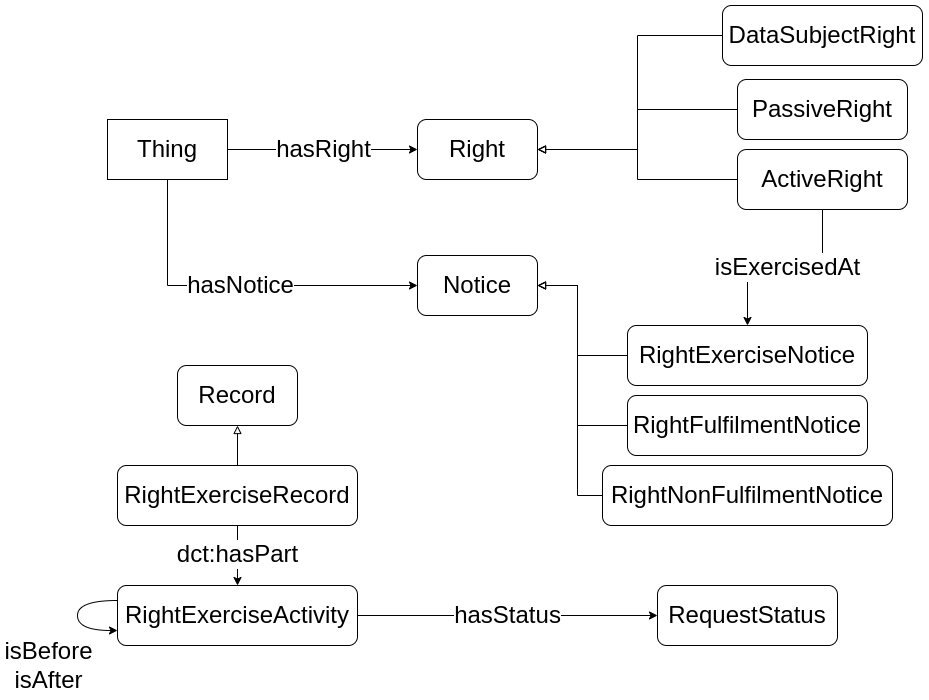
\includegraphics[width=0.8\linewidth]{figures/chapter-4/DPV-rights.png}
    \caption[Core concepts of DPV's rights taxonomy.]{Core concepts of DPV's rights taxonomy, adapted from \cite{pandit_primer_2022}.}
    \label{fig:rights_dpv}
\end{figure}

Thus, beyond modelling concepts for applicable \texttt{Right}s and \texttt{DataSubjectRight}s (applicable only to data subjects), to indicate the association of concepts with a particular right, the \texttt{hasRight} property is also modelled in DPV.
Additionally, to make a distinction between actionable and non-actionable rights, the \texttt{ActiveRight} and \texttt{PassiveRight} concepts were created to distinguish between rights that require an action to be taken for them to be exercised and rights that don't require any action and are always applicable.% add examples of active/passive rights
To fulfil the second objective of establishing where such active rights can be exercised, DPV's \texttt{isExercisedAt} property should be used to connect the right with the \texttt{RightExerciseNotice}.
This notice provides contextual information regarding how to exercise a right.
Specialised notice concepts for rights that can be fulfilled and those that cannot are modelled as \texttt{RightFulfilmentNotice} and \texttt{RightNonFulfilmentNotice}, respectively.

Moreover, to represent concrete records of rights being exercised, the \texttt{RightExerciseRecord} concept, specified as a subclass of DPV's \texttt{Record}, can be used to associate a particular request, or even distinct requests from the same data subject, with corresponding rights exercising activities, modelled as \texttt{RightExerciseActivity}, using the DCMI Metadata Terms \texttt{hasPart} property.
Such activity instances should include metadata, e.g., timestamps, duration, or involved entities, to track the provenance of a particular right exercising process, from the request itself to its acknowledgement by the data controller and to the fulfilment or non-fulfilment of the right.

In order to justify a certain right exercise activity, a collection of justifications for the non-fulfilment, i.e., \texttt{RightNonFulfilmentJustification}, delay of fulfilment, i.e.,\linebreak \texttt{RightFulfilmentDelayJustification}, and exercise of rights, i.e.,\linebreak \texttt{RightExerciseJustification}, were modelled as subclasses of the\linebreak \texttt{NonPerformanceJustification}, \texttt{DelayJustification}, and\linebreak \texttt{ExerciseJustification} concepts, which were modelled to have generic justification concepts that can be used beyond the rights domain.
\texttt{NotRequiredJustification}s are also modelled for when a certain request is not required as it does not apply. 
Figure~\ref{fig:justifications} contains the modelled justifications -- they are modelled as generic justifications to be included in DPV, which are then extended in DPV-GDPR by referencing specific GDPR clauses.
Moreover, the \texttt{dcterms:source} property will be used to connect the justification term with the GDPR provision that inspired its definition. 
These concepts have already been approved to be integrated into DPV and DPV-GDPR's outputs\footnote{Meeting notes of the DPVCG call where the concepts were accepted: \url{https://w3id.org/dpv/meetings/meeting-2024-03-13}.}.

\begin{figure}[ht]
    \centering
    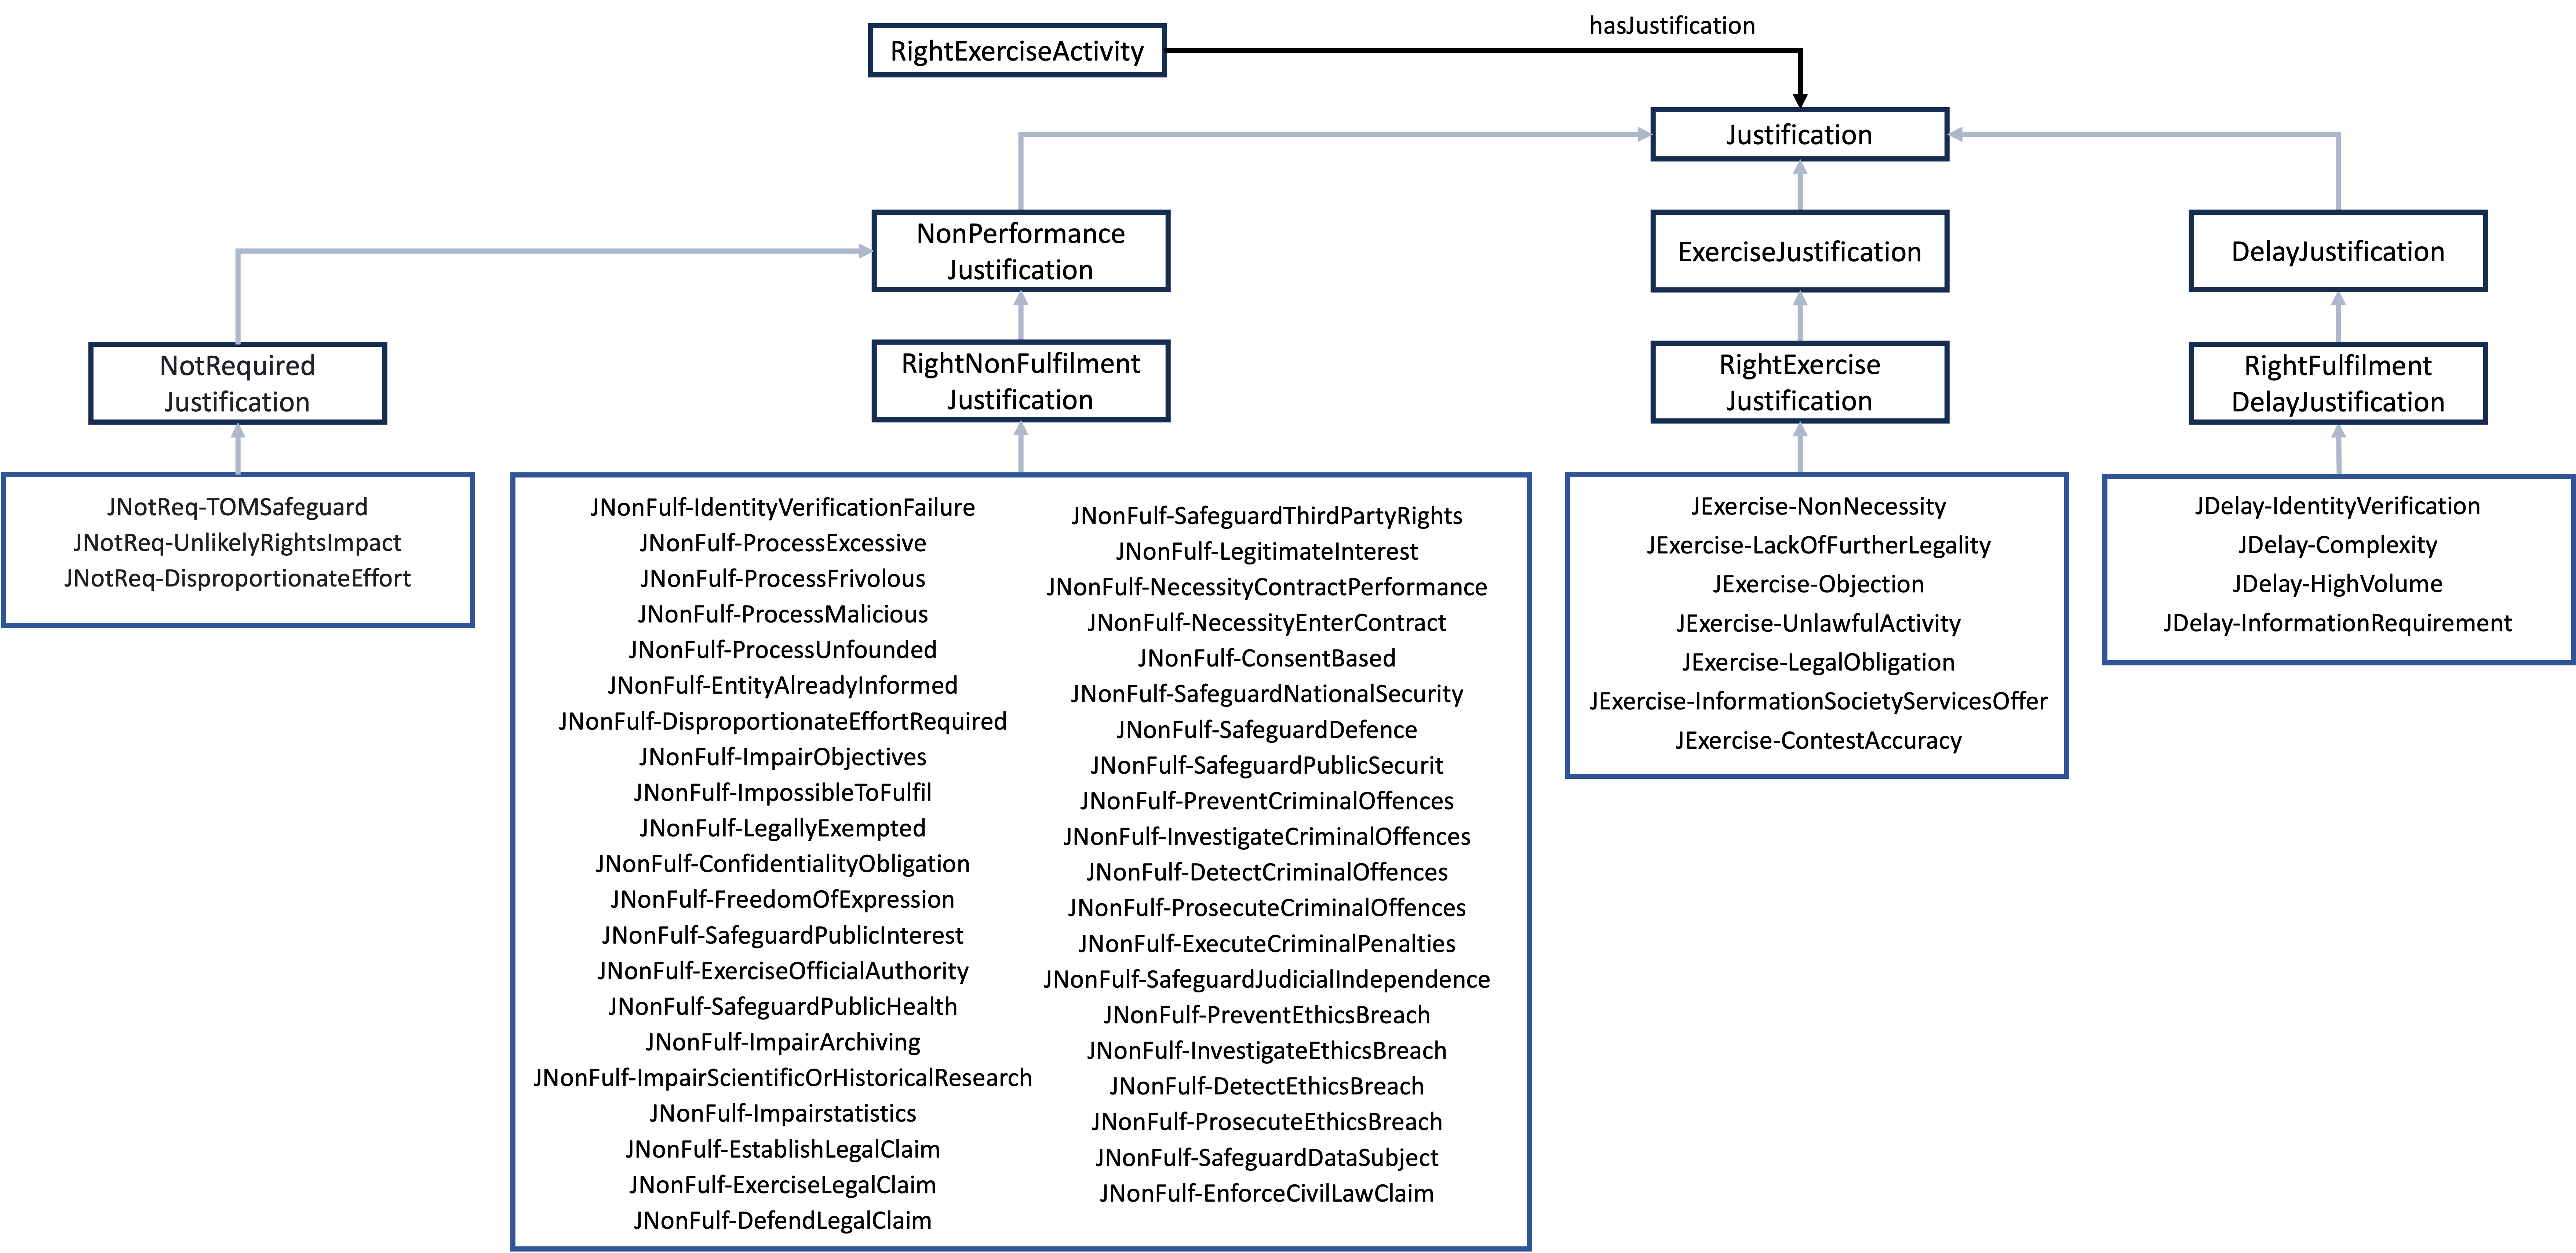
\includegraphics[width=\linewidth]{figures/chapter-4/justifications.png}
    \caption[Justification concepts.]{Justification concepts for the non-fulfilment, delay of fulfilment and exercise of rights.}
    \label{fig:justifications}
\end{figure}

Additionally, to track the status of rights exercising activities, a set of request statuses are modelled in DPV, including \texttt{RequestAccepted} for a request being accepted towards fulfilment, \texttt{RequestRejected} for a request being rejected towards non-fulfilment or\linebreak \texttt{RequestRequiresAction} for a request requiring an action to be performed from another party, and the \texttt{isBefore} and \texttt{isAfter} concepts can be used to specify that a specific activity occurs before or after another activity.

While this modelling was inspired by the GDPR, the concepts are described in a jurisdiction-agnostic manner so that they can be used to tackle data protection regulations in different jurisdictions.
For GDPR-specific rights, the \texttt{DataSubjectRight} concept is extended in DPV-GDPR with the data subject rights described in GDPR's Articles 13 to 22, as well as the rights to withdraw consent and to lodge a complaint with a supervisory authority, described in Articles 7.3 and 77.
Moreover, notices for direct and indirect data collection, to fulfil the information requirements in Articles 13 and 14, for Subject Access Requests (SARs), described in Article 15, and for notifying recipients, necessary to fulfil the communication requirements of Articles 16, 17 and 18, are provided as GDPR-specific subclasses of \texttt{RightFulfilmentNotice}s.

An overview of the aforementioned requirements and the intended purpose for modelling these concepts is presented in the ORSD illustrated in Table~\ref{tab:rights_ORSD}.

% also with these questions(in the ORSD) can you link directly to gdpr articles or other literature of gdpr implementation that help indicate these are valid requirements?

\begin{table}[htbp]
\centering
\caption{ORSD of the proposed model to express rights-related activities.}
\label{tab:rights_ORSD}
\scriptsize
\resizebox{\textwidth}{!}{%
\begin{tabular}{| l | l | l | l  | l | l | l |l| }
\hline
\multicolumn{8}{|c|}{\cellcolor[HTML]{A0A0A0}\textbf{Vocabulary-based patterns for rights exercising activities}} \\ \hline
\multicolumn{8}{|c|}{\cellcolor[HTML]{EFEFEF}\textbf{1. Purpose}} \\ \hline
\multicolumn{8}{| p{12.0cm} |}{The purpose of this model is the expression of rights-related activities, in particular focusing on data subject rights, such as the ones described in GDPR's Chapter III.} \\ \hline
\multicolumn{8}{|c|}{\cellcolor[HTML]{EFEFEF}\textbf{2. Scope}} \\ \hline
\multicolumn{8}{| p{12.0cm} |}{The scope of this model is limited to the expression of information related to the various steps of exercising data subject rights. In particular, the introduced concepts serve one of these purposes: (i) indicate what rights exist, (ii) express where such rights can be exercised, and (iii) record information related to concrete instances of rights that are being or were exercised. } \\ \hline
\multicolumn{8}{|c|}{\cellcolor[HTML]{EFEFEF}\textbf{3. Implementation Language}} \\ \hline
\multicolumn{8}{| p{12.0cm} |}{RDF, RDFS} \\ \hline
\multicolumn{8}{|c|}{\cellcolor[HTML]{EFEFEF}\textbf{4. Intended End-Users}} \\ \hline
\multicolumn{8}{| p{12.0cm} |}{Developers of Web services and applications, including decentralised storage solutions, that handle personal data.} \\ \hline
\multicolumn{8}{|c|}{\cellcolor[HTML]{EFEFEF}\textbf{5. Intended Uses}} \\ \hline
\multicolumn{8}{| p{12.0cm} |}{
Use 1. Declaration of the existence of data subject rights when the usage and collection of personal data is performed by Web services providers and developers, including information on where they can be exercised. \newline
Use 2. Patterns for data subject rights that can be fulfilled. \newline
Use 3. Patterns for data subject rights that cannot be fulfilled, including justifications for non-fulfilment. \newline
Use 4. Fulfilment of data subject rights requests from specific data protection legislation, such as the GDPR.
 } \\ \hline
\multicolumn{8}{|c|}{\cellcolor[HTML]{EFEFEF}\textbf{6. Ontology Requirements}} \\ \hline
\multicolumn{8}{|c|}{\cellcolor[HTML]{EFEFEF}\textbf{a. Non-Functional Requirements}}    \\ \hline
\multicolumn{8}{| p{12.0cm} |}{
NFR 1. The concepts are either published online within DPVCG's outputs, following W3C's specification format, or are under discussion for being adopted by the same CG. } \\ \hline
\multicolumn{8}{|c|}{\cellcolor[HTML]{EFEFEF}\textbf{b. Functional  Requirements: Groups of Competency Questions}}  \\ \hline
\multicolumn{5}{|c|}{\cellcolor[HTML]{EFEFEF}CQRG1. Related to data subject rights} & \multicolumn{3}{|c|}{\cellcolor[HTML]{EFEFEF}CQRG2. Related to GDPR} \\ \hline
\multicolumn{5}{ | m{7cm} |}{
CQR1. What rights are applicable in a given context? \newline
CQR2. Where can the right be exercised? \newline
CQR3. How can the right be exercised? \newline
CQR4. What data is necessary to implement the right? \newline 
CQR5. Which entity implements the right? \newline 
CQR6. Which entity exercised the right? \newline 
CQR7. When is the exercising activity occurring? \newline 
CQR8. What is the status of the right request? } & 
\multicolumn{3}{ m{5cm} |}{
CQR9. Which data subject rights are applicable according to the legal basis used by the data controller? \newline
CQR10. Which provenance metadata must controllers provide when replying to data subject rights requests? \newline 
CQR11. Which justification can be provided to not fulfil, delay or exercise a request?
}\\ \hline
\end{tabular}}
\vspace{-0.1in}
\end{table}

\subsection{Vocabulary-based patterns for rights exercising activities}
\label{sec:rights_patterns}

This Section outlines the usage of DPV for the expression of rights exercising activities, specifically related to the data subject rights described in GDPR's Chapter III.
Accordingly, the \textit{``controller shall take appropriate measures to provide any information referred to in Articles 13 and 14 and any communication under Articles 15 to 22 [...] to the data subject in a concise, transparent, intelligible and easily accessible form''} and if \textit{``the data subject makes the request by electronic form means, the information shall be provided by electronic means where possible, unless otherwise requested by the data subject''} \citeyearpar{noauthor_regulation_2016}.
Consequently, in this Thesis, personal data processing-related vocabularies such as DPV, and other semantic metadata vocabularies such as DCMI Metadata Terms and DCAT, are used for the establishment of structured notices and records of activities, which promote the fulfilment of the transparency and machine-readability requirements previously described.
Additionally, by storing such information in decentralised personal datastores, the accessibility requirement can also be satisfied.

Listing~\ref{list:applicable_rights} provides an example of a personal data handling activity, which can be used to express information regarding the what, how, where, who, and why personal data is being processed, as well as what rights exist.
The example provides information regarding the type of personal data, \texttt{pd:EmailAddress}, being processed by the \texttt{ex:DataController}, the purpose and legal basis used for the processing to occur, \texttt{dpv:ServiceProvision} and \texttt{eu-gdpr:A6-1-a}, and the applicable GDPR data subject rights.
This pattern can be followed by data controllers to express which rights are applicable, including rights beyond the ones in the GDPR, e.g., EU's fundamental rights and the rights depicted in other EU regulations or in other jurisdictions.

\begin{listing}[htp]
\caption[Personal data handling activity with applicable rights.]{Personal data handling activity example which includes information regarding the applicable rights.}
\label{list:applicable_rights}
\begin{minted}{turtle}
ex:ProcessEmailForServiceProvision a dpv:PersonalDataHandling ;
    dpv:hasDataController ex:DataController ;
    dpv:hasPersonalData pd:EmailAddress ;
    dpv:hasProcessing dpv:Collect, dpv:Use ;
    dpv:hasPurpose dpv:ServiceProvision ;
    dpv:hasLegalBasis eu-gdpr:A6-1-a ;
    dpv:hasRight eu-gdpr:A7-3, eu-gdpr:A13, eu-gdpr:A14, eu-gdpr:A15, eu-gdpr:A16, eu-gdpr:A17, eu-gdpr:A18, eu-gdpr:A20, eu-gdpr:A22, eu-gdpr:A77 .
ex:DataController a dpv:DataController .
\end{minted}
\end{listing}

Moreover, such declarations of applicable rights should include a notice of where they can be exercised.
Thus, as described in the previous Section, DPV’s \texttt{isExercisedAt} property should be used to connect rights with information on where to exercise it.
Such information should be provided through a \texttt{RightExerciseNotice}, along with other rights exercising metadata.

Listing~\ref{list:exercise_point} provides a notice with information on where to exercise the GDPR's right of access related to personal data being processed by the \texttt{ex:DataController}.
This notice uses the \texttt{dpv:hasRight} property to indicate which rights can be exercised, beyond the already mentioned access right, and the \texttt{foaf:page} property to express the precise Web page where the right can be exercised.
Additionally, DPV's \texttt{hasDataController} and\linebreak \texttt{isImplementedByEntity} properties are used to define who is the controller responsible for the personal data being processed and who is the entity implementing the service/platform where the rights are exercised -- in most cases this entity will probably coincide with the data controller, however, for transparency and accountability purposes, it is reasonable to express both terms.
Other entity-related properties can also be used to personalise the notice, e.g., if a notice is personalised for a specific data subject, then \texttt{dpv:hasDataSubject} can be used to connect the notice with the individual data subject. 
Furthermore, personal data handling instances can also be used to express `data processing bundles' that need to be provided in order to fulfil the data subjects' rights.
As previously mentioned, this can be done using DPV's taxonomies of purposes, personal data categories, processing operations, etc, e.g., in Listing~\ref{list:exercise_point}, an account identifier is required by the data controller for identity verification purposes in order to fulfil the data subject's rights described in GDPR's Articles 7.3, 15, 16, 17 and 20.
Other information might be needed to be communicated to the user, for instance, information on payments as Article 12.5(a) states that a fee \textit{``taking into account the administrative costs of providing the information or communication or taking the action requested''} might be requested by the data controller in case the data subject's request is unfounded, excessive or repetitive.
Such information can also be expressed in personal data handling instances including ODRL policies with duties constrained with an \texttt{odrl:payAmount} left operand.
% need to be provided / are being provided

\begin{listing}[htp]
\caption[GDPR Article 15's right of access exercise notice.]{GDPR Article 15's right of access exercise notice, including information on where to exercise the right and on necessary data to fulfil the right.}
\label{list:exercise_point}
\begin{minted}{turtle}
ex:RightToAccess a eu-gdpr:A15 ;
    dpv:isExercisedAt ex:RightExercisePoint .

ex:RightExercisePoint a dpv:RightExerciseNotice ;
    dpv:hasRight eu-gdpr:A7-3, eu-gdpr:A15, eu-gdpr:A16, eu-gdpr:A17, eu-gdpr:A20 ;
    dpv:hasDataController ex:DataController ;
    dpv:isImplementedByEntity ex:DataController ;
    foaf:page <https://example.com/DataController/RightExercisePoint> ;
    dpv:hasPersonalDataHandling [ 
        a dpv:PersonalDataHandling ;
        dpv:hasPurpose dpv:IdentityVerification ;
        dpv:hasPersonalData pd:AccountIdentifier ;
        dpv:hasProcessing dpv:Collect, dpv:Store ;
        dpv:hasRecipientDataController ex:DataController ] .
\end{minted}
\end{listing}

In addition to notices expressing what rights are applicable and where they can be exercised, provenance metadata must be kept when actual instances of the rights are exercised, throughout the whole process, from initiating a request to rejecting or fulfilling it.
As such, DPV's \texttt{RightExerciseActivity} can be used in conjunction with the W3C's PROV-O recommendation~\citep{lebo_prov-o_2013} to track the provenance of a right exercising activity instance.
Using this standard, provenance information, regarding the entities whom the request is associated with, i.e., \texttt{prov:wasAssociatedWith}, or what data/notice was generated, i.e., \texttt{prov:generated}, by the right exercise activity, can be represented.
\texttt{prov:actedOnBehalfOf} can also be used to represent delegation or representation, for instance when a parent exercises a right on behalf of its child.
Temporal information, descriptions and identifiers of the activities and their creators/publishers can be recorded using DCMI Metadata Terms.
Connections to the previous or following activities can be done using the \texttt{dpv:isAfter} and \texttt{dpv:isBefore} concepts, respectively.
Moreover, to track the status of a right exercising activity, DPV's taxonomy of request statuses concepts can be used.

Figure~\ref{fig:request_status} illustrates the sequence in which these concepts occur.
Once the request is initiated, it should be then acknowledged by the entity implementing it and either accepted towards fulfilment or rejected towards non-fulfilment.
Additionally, after being rejected, the entity fulfilling the request can also require further action from the requester (e.g., request additional data to be able to fulfil the request), which can delay the acceptance or rejection of the request, and after the required action is performed, the request can either be accepted towards fulfilment or get rejected again towards non-fulfilment or towards asking again for further action.

% perhaps formalise the semantics a bit more using uml state machine notation?
\begin{figure}[htp]
    \centering
    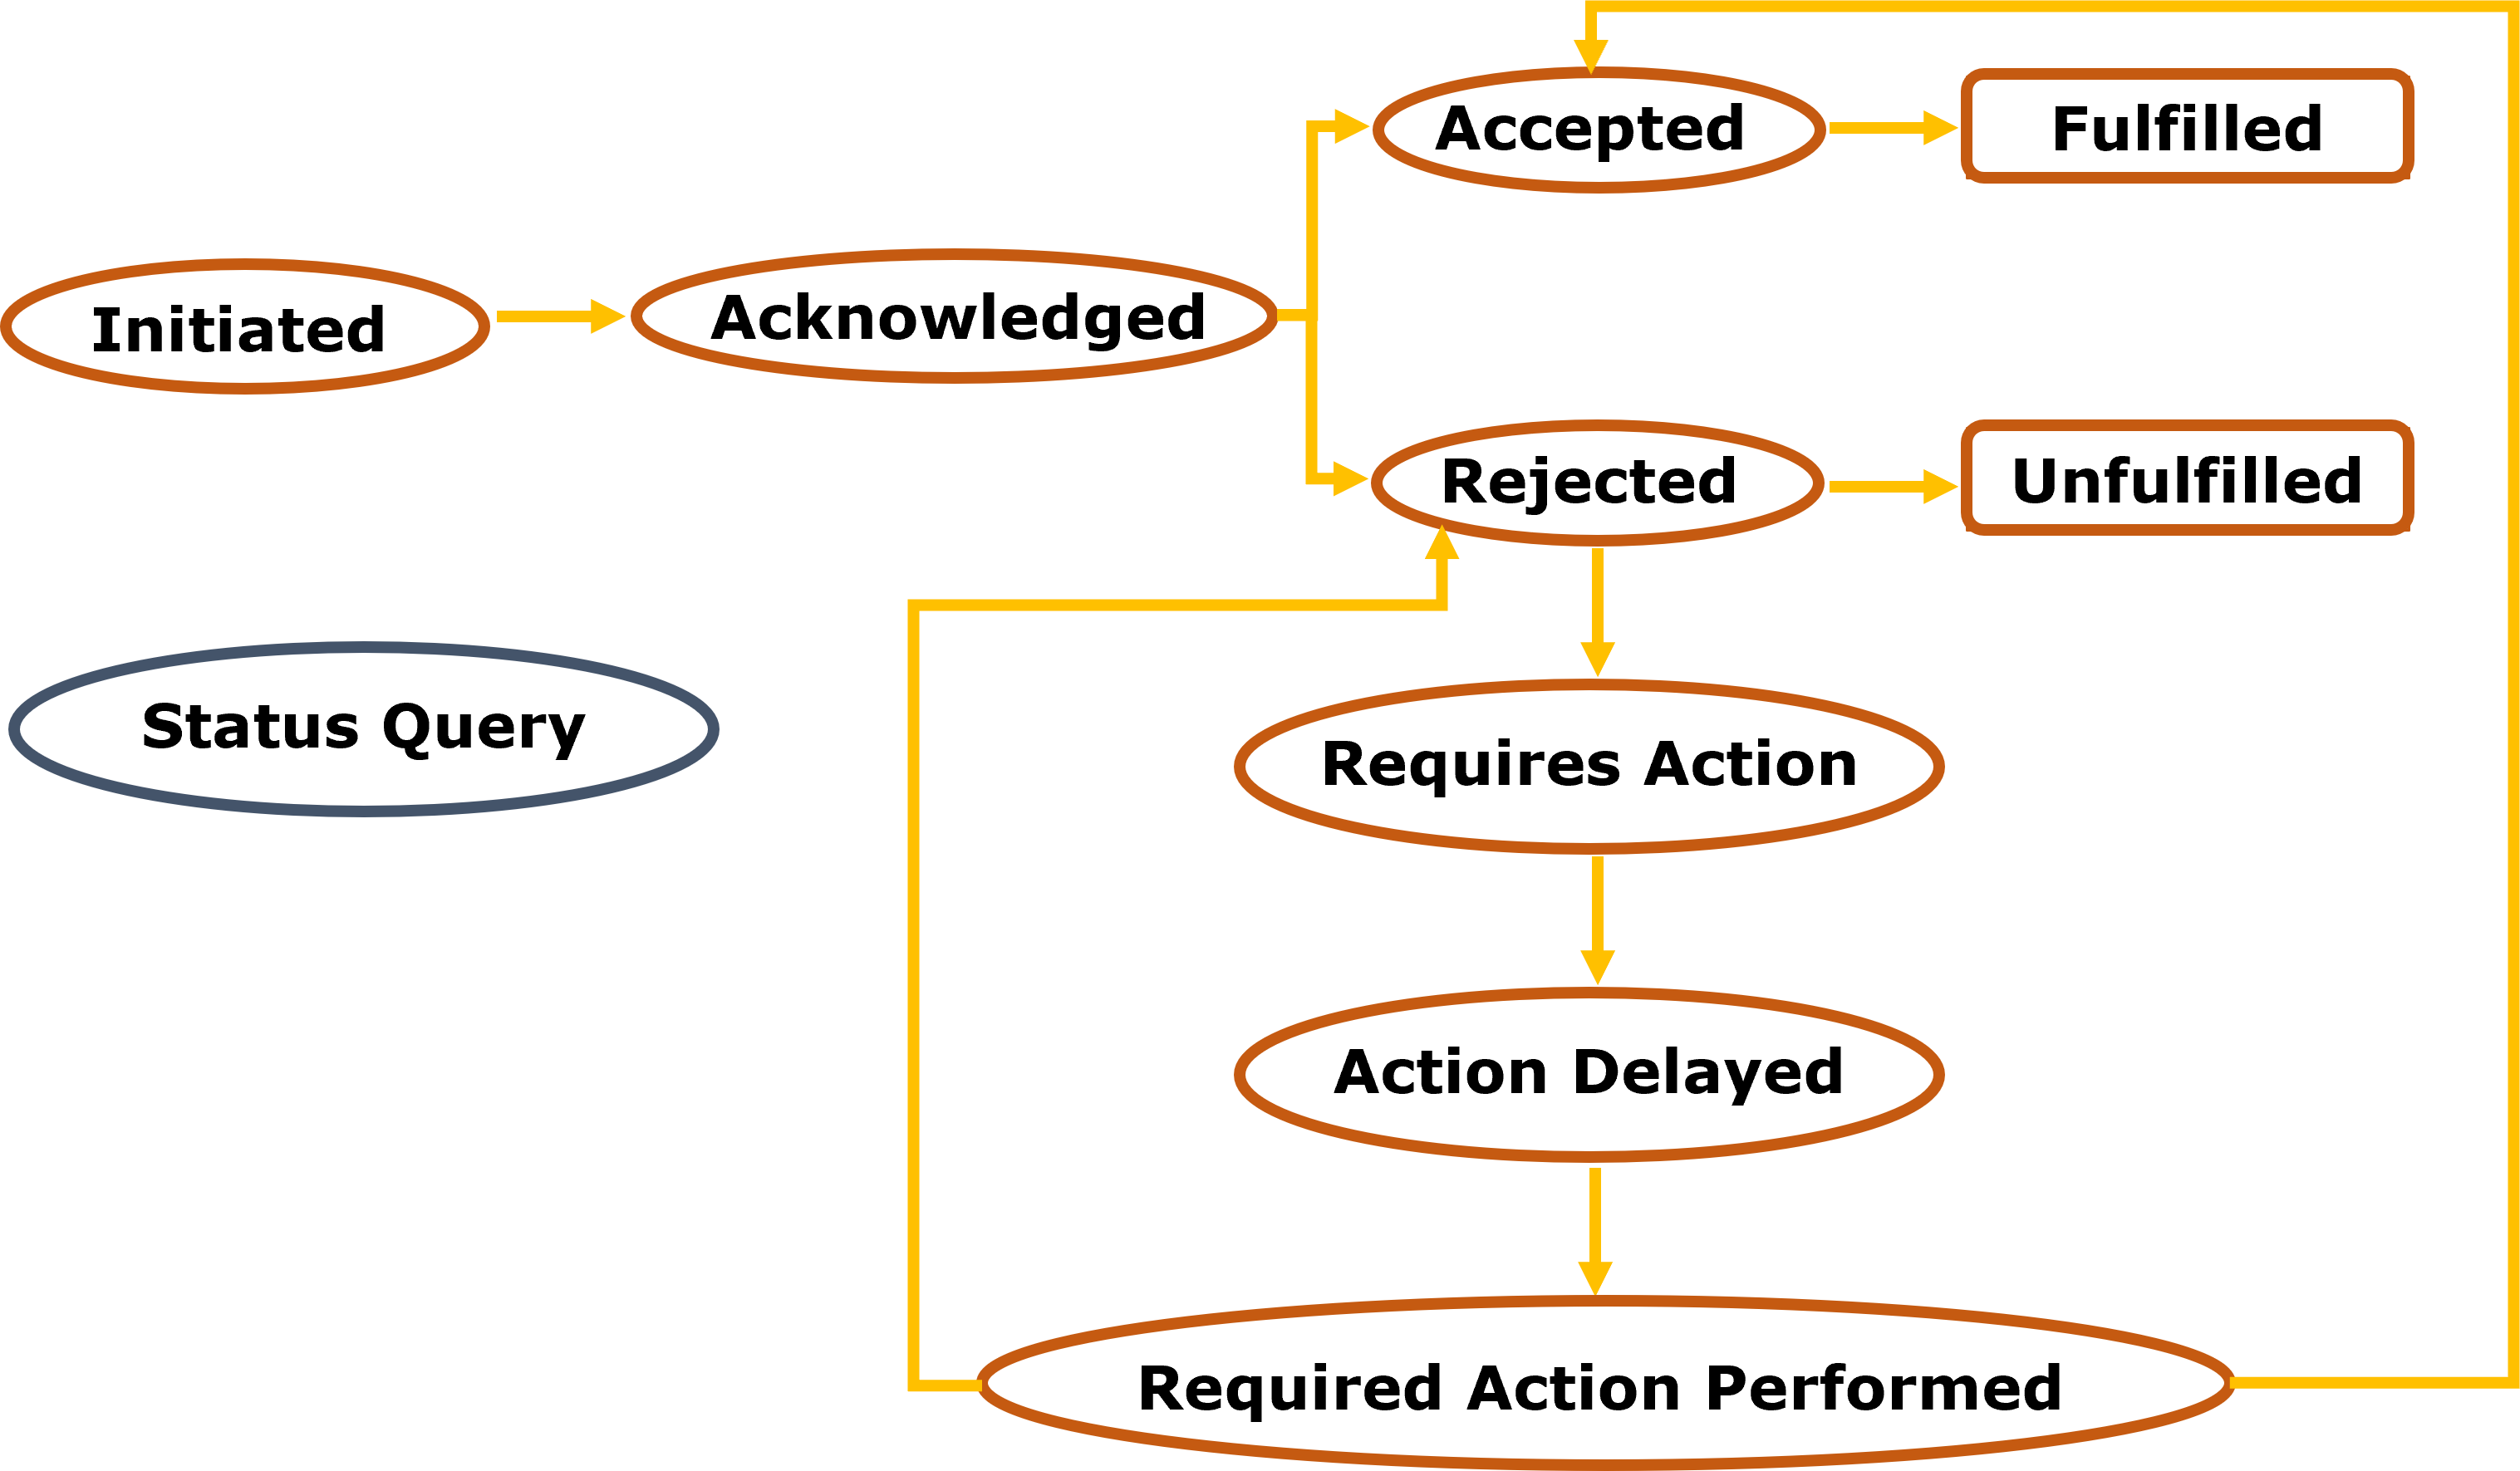
\includegraphics[width=0.8\linewidth]{figures/chapter-4/request-status.png}
    \caption{DPV's concepts to model the status of a request.}
    \label{fig:request_status}
\end{figure}

Listing~\ref{list:request_acknowledgment} illustrates a record of the right exercising activities related to a GDPR right of access request and acknowledgement of said request.
The activity associated with the start of the request has the status \texttt{dpv:RequestInitiated}, the data subject is identified using the \texttt{dpv:hasDataSubject} and the recipient of the request, a data controller, using the \texttt{dpv:hasRecipientDataController}.
Furthermore, a personal data handling instance can be used to express what personal data needs to be processed for the fulfilment of the right and DPV's \texttt{hasScope} to specify the scope of the request, e.g., the data subject only wants to access data processed for service provision purposes or only data processed during 2022.
Following the start of the request, the controller acknowledges the request, a right exercising activity which has \texttt{dpv:RequestAcknowledged} status and the recipient is the data subject that initiated the request.

\begin{listing}[htp]
\caption{Record of GDPR right of access request and acknowledgement activities.}
\label{list:request_acknowledgment}
\begin{minted}{turtle}
ex:DataSubject a dpv:DataSubject .
ex:DataSubjectUsername a pd:AccountIdentifier ;
    dpv:hasDataSubject ex:DataSubject .

ex:SARequest a dpv:RightExerciseActivity, prov:Activity ;
    dcterms:description "Data Subject makes a GDPR right of access request" ;
    dpv:hasRight eu-gdpr:A15 ;
    dpv:isExercisedAt ex:RightExercisePoint ;
    prov:wasAssociatedWith ex:DataSubject ;
    dpv:hasDataSubject ex:DataSubject ;
    dpv:hasRecipientDataController ex:DataController ;
    dcterms:date "2023-11-02T11:08:05"^^xsd:dateTime ;
    dpv:hasStatus dpv:RequestInitiated ;
    dpv:hasPersonalDataHandling [
        a dpv:PersonalDataHandling ;
        dpv:hasPurpose dpv:IdentityVerification ;
        dpv:hasPersonalData ex:DataSubjectUsername ;
        dpv:hasProcessing dpv:Collect, dpv:Store ] ;
    dpv:hasScope [
        dpv:hasPurpose dpv:ServiceProvision ;
        dpv:hasDuration [
            time:hasBeginning "2022-01-01T00:00:00"^^xsd:dateTime ;
            time:hasEnd "2022-12-31T23:59:59"^^xsd:dateTime ] ] .

ex:SARAcknowledged a dpv:RightExerciseActivity, prov:Activity ;
    dcterms:description "Data controller acknowledges the request" ;
    dcterms:date "2023-11-02T15:55:10"^^xsd:dateTime ;
    prov:wasAssociatedWith ex:DataController ;
    dpv:hasRecipient ex:DataSubjectUsername ;
    dpv:hasStatus dpv:RequestAcknowledged ;
    dpv:isAfter ex:SARequest .
\end{minted}
\end{listing}

Listing~\ref{list:further_action} illustrates the follow-up to Listing~\ref{list:request_acknowledgment} -- the request was rejected\linebreak due to the data controller not being able to identify the data subject,\linebreak \texttt{JNonFulf-IdentityVerificationFailure}.
Table~\ref{tab:justifications} contains the list of modelled right non-fulfilment justifications and their labels, which can be used by controllers for the purpose of justifying such requests.
As such the data controller requires further information from the data subject to be able to proceed with the request.
Such right exercise activity is identified with the \texttt{dpv:RequestRequiresAction} status and contains a personal data handling activity instance expressing the information that the data subject needs to provide for the right exercise to continue.
Afterwards, a right exercise activity associated with the data subject and with a \texttt{dpv:RequestRequiredActionPerformed} status is recorded with the information that the data subject provided.

\begin{listing}[htp]
\caption[Record requesting further information to fulfil SAR.]{Record of data controller requesting further information to fulfil the data subject's SAR and of the data subject providing the controller with said information.}
\label{list:further_action}
\begin{minted}{turtle}
ex:SARRejected a dpv:RightExerciseActivity, prov:Activity;
    dcterms:description "Data controller rejects the request" ;
    dcterms:date "2023-11-02T15:57:31"^^xsd:dateTime ;
    prov:wasAssociatedWith ex:DataController ;
    dpv:hasRecipient ex:DataSubjectUsername ;
    dpv:hasStatus dpv:RequestRejected ;
    dpv:hasJustification justif:JNonFulf-IdentityVerificationFailure ;
    dpv:isAfter ex:SARAcknowledged .

ex:SARRequiresAction a dpv:RightExerciseActivity, prov:Activity ;
    dcterms:description "Data controller requires further actions" ;
    dcterms:date "2023-11-02T16:09:21"^^xsd:dateTime ;
    prov:wasAssociatedWith ex:DataController ;
    dpv:hasRecipient ex:DataSubjectUsername ;
    dpv:hasStatus dpv:RequestRequiresAction ;
    dpv:hasJustification justif:JNonFulf-IdentityVerificationFailure ;
    dpv:hasPersonalDataHandling [
        dpv:hasPersonalData pd:OfficialID ;
        dpv:hasProcessing dpv:MakeAvailable ;
        dpv:hasPurpose dpv:IdentityVerification ;
        dpv:hasRecipientDataController ex:DataController ;
        dpv:isImplementedByEntity ex:DataSubjectUsername ] ;
    dpv:isAfter ex:SARRejected .

ex:DataSubjectOfficialID a pd:OfficialID ;
    dpv:hasDataSubject ex:DataSubject .

ex:SARActionPerformed a dpv:RightExerciseActivity, prov:Activity ;
    dcterms:description "Data Subject provides required information" ;
    dcterms:date "2023-11-02T17:20:42"^^xsd:dateTime ;
    prov:wasAssociatedWith ex:DataSubject ;
    dpv:hasStatus dpv:RequestRequiredActionPerformed ;
    dpv:hasPersonalDataHandling [
        dpv:hasPersonalData ex:DataSubjectOfficialID ;
        dpv:hasProcessing dpv:MakeAvailable ;
        dpv:hasPurpose dpv:IdentityVerification ;
        dpv:hasRecipientDataController ex:DataController ;
        dpv:isImplementedByEntity ex:DataSubjectUsername ] ;
    dpv:isAfter ex:SARRequiresAction .
\end{minted}
\end{listing}

% rights non-fulfilment justifications issue: https://github.com/w3c/dpv/issues/63 & meeting minutes:https://www.w3.org/2022/10/19-dpvcg-minutes.html
\begin{landscape}
\begin{table}
    \centering
    \caption{Justifications for non-fulfilment of GDPR's data subject rights.}
    \label{tab:justifications}
    \resizebox{\textwidth}{!}{%
    \begin{tabular}{c|l|c}
        \textbf{Term} & \textbf{Label} & \multicolumn{1}{c}{\begin{tabular}[c]{@{}c@{}} \textbf{GDPR} \\ \textbf{Article(s)} \end{tabular}} \\
        \hline\hline
        \texttt{JNonFulf-IdentityVerificationFailure} & \multicolumn{1}{l|}{\begin{tabular}[l]{@{}l@{}} Justification that the process could not be fulfilled or was not successful\\ because identity verification failed \end{tabular}} & 12.2 \\
        \hline
        \texttt{JNonFulf-ProcessExcessive} & Request was excessive in scope & 12.5 \\
        \hline
        \texttt{JNonFulf-ProcessFrivolous} & Request was frivolous in scope & 12.5 \\
        \hline
        \texttt{JNonFulf-ProcessMalicious} & Request was malicious in scope & 12.5 \\
        \hline
        \texttt{JNonFulf-ProcessUnfounded} & Request was unfounded in scope & 12.5 \\
         \hline
        \texttt{JNonFulf-EntityAlreadyInformed} & \multicolumn{1}{l|}{\begin{tabular}[l]{@{}l@{}} Data subject already has been provided with this information \end{tabular}} & 13.4, 14.5(a) \\
         \hline
        \texttt{JNonFulf-ImpairObjectives} & Fulfilment would cause impairment to processing & 14.5(b) \\
        \hline     
        \texttt{JNonFulf-DisproportionateEffortRequired} & Fulfilment would require extraordinary effort & 14.5(b), 19 \\
         \hline
        \texttt{JNonFulf-ImpossibleToFulfil} & Fulfilment would be impossible & 14.5(b), 19 \\
         \hline
        \texttt{JNonFulf-LegallyExempted} & \multicolumn{1}{l|}{\begin{tabular}[l]{@{}l@{}} Fulfilment not needed as it falls under legal exemption \end{tabular}} & \multicolumn{1}{l}{\begin{tabular}[l]{@{}l@{}} 14.5(c), 17.3(b),\\ 22.2(b) \end{tabular}} \\
         \hline
        \texttt{JNonFulf-ConfidentialityObligation} & \multicolumn{1}{l|}{\begin{tabular}[l]{@{}l@{}} Fulfilment would compromise existing confidentiality obligations \end{tabular}} & 14.5(d) \\
        \hline
        \texttt{JNonFulf-FreedomOfExpression} & \multicolumn{1}{l|}{\begin{tabular}[l]{@{}l@{}} Fulfilment would interfere with the right of freedom of expression\\ and information of others \end{tabular}} & 17.3(a) \\
         \hline
        \texttt{JNonFulf-SafeguardPublicInterest} & \multicolumn{1}{l|}{\begin{tabular}[l]{@{}l@{}} Fulfilment would interfere with necessary tasks carried out for public\\ interest \end{tabular}} & \multicolumn{1}{l}{\begin{tabular}[l]{@{}l@{}} 17.3(b), 21.6,\\ 23.1(e) \end{tabular}} \\
         \hline
         \texttt{JNonFulf-ExerciseOfficialAuthority} & \multicolumn{1}{l|}{\begin{tabular}[l]{@{}l@{}} Fulfilment would interfere with the exercise of official authorities \end{tabular}} & \multicolumn{1}{l}{\begin{tabular}[l]{@{}l@{}} 17.3(b), 20.3,\\ 23.1(h) \end{tabular}} \\
         \hline
         \texttt{JNonFulf-SafeguardPublicHealth} & \multicolumn{1}{l|}{\begin{tabular}[l]{@{}l@{}} Fulfilment would interfere with necessary tasks carried out for public\\ health reasons \end{tabular}} & 17.3(c) \\
         \hline
        \texttt{JNonFulf-ImpairArchiving} & \multicolumn{1}{l|}{\begin{tabular}[l]{@{}l@{}} Fulfilment would compromise or hinder archiving purposes \end{tabular}} & 17.3(d) \\
        \hline
        \texttt{JNonFulf-ImpairScientificOrHistoricalResearch} & \multicolumn{1}{l|}{\begin{tabular}[l]{@{}l@{}} Fulfilment would impair scientific or historical research \end{tabular}} & 17.3(d) \\
        \hline
        \texttt{JNonFulf-ImpairStatistics} & \multicolumn{1}{l|}{\begin{tabular}[l]{@{}l@{}} Fulfilment would interfere with official statistics \end{tabular}} & 17.3(d) \\
        \hline
        \texttt{JNonFulf-EstablishLegalClaim} & \multicolumn{1}{l|}{\begin{tabular}[l]{@{}l@{}} Fulfilment would interfere with the establishment of legal claims \end{tabular}} & 17.3(e), 21.1 \\
        \hline
        \texttt{JNonFulf-ExerciseLegalClaim} & \multicolumn{1}{l|}{\begin{tabular}[l]{@{}l@{}} Fulfilment would interfere with the exercise of legal claims \end{tabular}} & 17.3(e), 21.1 \\
        \hline
        \texttt{JNonFulf-DefendLegalClaim} & \multicolumn{1}{l|}{\begin{tabular}[l]{@{}l@{}} Fulfilment would interfere with the defence of legal claims \end{tabular}} & 17.3(e), 21.1 \\
        \hline
        \texttt{JNonFulf-SafeguardThirdPartyRights} & \multicolumn{1}{l|}{\begin{tabular}[l]{@{}l@{}} Fulfilment would adversely affect the rights of other data subjects or third\\ parties \end{tabular}} & 20.4, 23.1(i) \\
         \hline
         \texttt{JNonFulf-LegitimateInterest} & \multicolumn{1}{l|}{\begin{tabular}[l]{@{}l@{}} Fulfilment would interfere with the legitimate interest of the controller\\ which overrides the interests or rights of the data subject \end{tabular}} & 21.1 \\
         \hline
        \texttt{JNonFulf-NecessityContractPerformance} & \multicolumn{1}{l|}{\begin{tabular}[l]{@{}l@{}} Fulfilment would interfere with the performance of a contract \end{tabular}} & 22.2(a) \\
         \hline
        \texttt{JNonFulf-NecessityEnterContract} & \multicolumn{1}{l|}{\begin{tabular}[l]{@{}l@{}} Fulfilment would interfere with the necessity of entering into a contract \end{tabular}} & 22.2(a) \\
         \hline
        \texttt{JNonFulf-ConsentBased} & \multicolumn{1}{l|}{\begin{tabular}[l]{@{}l@{}} Fulfilment not necessary as processing is based on explicit consent \end{tabular}} & 22.2(c) \\
        \hline
        \texttt{JNonFulf-SafeguardNationalSecurity} & \multicolumn{1}{l|}{\begin{tabular}[l]{@{}l@{}} Fulfilment would pose a threat to safeguard national security \end{tabular}} & 23.1(a) \\
         \hline
        \texttt{JNonFulf-SafeguardDefence} & Fulfilment would pose a threat to safeguard defence & 23.1(b) \\
         \hline
        \texttt{JNonFulf-SafeguardPublicSecurity} & \multicolumn{1}{l|}{\begin{tabular}[l]{@{}l@{}} Fulfilment would pose a threat to safeguard public security \end{tabular}} & 23.1(c) \\
         \hline
        \texttt{JNonFulf-PreventCriminalOffences} & \multicolumn{1}{l|}{\begin{tabular}[l]{@{}l@{}} Fulfilment would interfere with the prevention of criminal offences \end{tabular}} & 23.1(d) \\
        \hline
        \texttt{JNonFulf-InvestigateCriminalOffences} & \multicolumn{1}{l|}{\begin{tabular}[l]{@{}l@{}} Fulfilment would interfere with the investigation of criminal offences \end{tabular}} & 23.1(d) \\
        \hline
        \texttt{JNonFulf-DetectCriminalOffences} & \multicolumn{1}{l|}{\begin{tabular}[l]{@{}l@{}} Fulfilment would interfere with the detection of criminal offences \end{tabular}} & 23.1(d) \\
        \hline
        \texttt{JNonFulf-ProsecuteCriminalOffences} & \multicolumn{1}{l|}{\begin{tabular}[l]{@{}l@{}} Fulfilment would interfere with the prosecution of criminal offences \end{tabular}} & 23.1(d) \\
        \hline
        \texttt{JNonFulf-ExecuteCriminalPenalties} & \multicolumn{1}{l|}{\begin{tabular}[l]{@{}l@{}} Fulfilment would interfere with the execution of criminal penalties \end{tabular}} & 23.1(d) \\
        \hline
        \texttt{JNonFulf-SafeguardJudicialIndependence} & \multicolumn{1}{l|}{\begin{tabular}[l]{@{}l@{}} Fulfilment would pose a threat to safeguard judicial independence or\\ proceedings \end{tabular}} & 23.1(f) \\
        \hline
        \texttt{JNonFulf-PreventEthicsBreach} & \multicolumn{1}{l|}{\begin{tabular}[l]{@{}l@{}} Fulfilment would interfere with the prevention of breaches of ethics for\\ regulated professions \end{tabular}} & 23.1(g) \\
        \hline
        \texttt{JNonFulf-InvestigateEthicsBreach} & \multicolumn{1}{l|}{\begin{tabular}[l]{@{}l@{}} Fulfilment would interfere with the investigation of breaches of ethics for\\ regulated professions \end{tabular}} & 23.1(g) \\
        \hline
        \texttt{JNonFulf-DetectEthicsBreach} & \multicolumn{1}{l|}{\begin{tabular}[l]{@{}l@{}} Fulfilment would interfere with the detection of breaches of ethics for\\ regulated professions \end{tabular}} & 23.1(g) \\
        \hline
        \texttt{JNonFulf-ProsecuteEthicsBreach} & \multicolumn{1}{l|}{\begin{tabular}[l]{@{}l@{}} Fulfilment would interfere with the prosecution of breaches of ethics for\\ regulated professions \end{tabular}} & 23.1(g) \\
        \hline
        \texttt{JNonFulf-SafeguardDataSubject} & \multicolumn{1}{l|}{\begin{tabular}[l]{@{}l@{}} Fulfilment would interfere with the protection of the data subject \end{tabular}} & 23.1(i) \\
         \hline
        \texttt{JNonFulf-EnforceCivilLawClaim} & Fulfilment would interfere with the enforcement of civil law claims & 23.1(j) \\
    \end{tabular}}
\end{table}
\end{landscape}
% Information is legally exempt from disclosure	- Documents that have personal data of the data subject exempt from disclosure in court proceedings apply in relation to a Subject Access Request, this applies to both legal advice and litigation privilege

Listing~\ref{list:sar_notice} illustrates the follow-up to Listing~\ref{list:further_action} -- the request was accepted and fulfilled by the data controller and as such the data controller provides the data subject with a notice of the fulfilment of GDPR's Art.15, modelled as a \texttt{eu-gdpr:SARNotice}, and a copy of the data whose access was requested, modelled as a \texttt{dcat:Dataset}.
Beyond temporal information and providing the location of the notice, a personal data handling instance can be used to provide additional information to the data subject -- in the case of this SAR notice, the data subject is also notified of the type of personal data being processed, the purpose for the processing, the time period when the data was processed and the additional data subject rights that can be exercised.

\begin{listing}[htp]
\caption[Record of the acceptance and fulfilment of a SAR request.]{Record of the acceptance and fulfilment of the request and respective \texttt{SARNotice}.}
\label{list:sar_notice}
\begin{minted}{turtle}
ex:SARAccepted a dpv:RightExerciseActivity, prov:Activity ;
    dcterms:description "Request accepted by data controller towards fulfilment" ;
    dcterms:date "2023-11-03T08:15:04"^^xsd:dateTime ;
    prov:wasAssociatedWith ex:DataController ;
    dpv:hasRecipient ex:DataSubjectUsername ;
    dpv:hasStatus dpv:RequestAccepted ;
    dpv:isAfter ex:SARActionPerformed .

ex:SARFulfilled a dpv:RightExerciseActivity, prov:Activity ;
    dcterms:description "Request fulfilled by data controller" ;
    dcterms:date "2023-11-03T08:37:25"^^xsd:dateTime ;
    prov:wasAssociatedWith ex:DataController ;
    dpv:hasRecipient ex:DataSubjectUsername ;
    dpv:hasStatus dpv:RequestFulfilled ;
    prov:generated ex:DataCopy, ex:SARNotice_Username ;
    dpv:isAfter ex:SARAccepted .

ex:SARNotice_Username a eu-gdpr:SARNotice ;
    dcterms:date "2023-11-03T08:31:51"^^xsd:dateTime ;
    foaf:page <https://example.com/DataController/SARNotice_Username> ;
    dpv:hasPersonalDataHandling [
        dpv:hasPersonalData pd:EmailAddress ;
        dpv:hasPurpose dpv:ServiceProvision ;
        dpv:hasDuration [
            time:hasBeginning "2022-01-01T00:00:00"^^xsd:dateTime ;
            time:hasEnd "2022-12-31T23:59:59"^^xsd:dateTime ] ;
        dpv:hasRight eu-gdpr:A16, eu-gdpr:A17, eu-gdpr:A18, eu-gdpr:A21, eu-gdpr:A77 ] .

ex:DataCopy a dcat:Dataset ;
    dcterms:format <https://www.iana.org/assignments/media-types/text/csv> ;
    dcterms:accessRights access-right:c_16ec ; # restricted access
    dcterms:issued "2023-11-03T08:35:42"^^xsd:dateTime ;
    dcterms:valid "2023-12-03T08:35:42"^^xsd:dateTime ;
    dcat:landingPage <https://example.com/Username/SAR_DataCopy> .
\end{minted}
\end{listing}

Moreover, DCAT \citep{albertoni_data_2020} can be used to model resources beyond notices, for instance, a copy of the personal data, in the case of a right of access request according to the GDPR, as in Listing~\ref{list:sar_notice}.
Information regarding the format, validity and dataset provision/download location can be attached to the dataset representation using the \texttt{dcterms:format}, \texttt{dcterms:valid} and \texttt{dcat:landingPage} properties, respectively.
Additionally, DCAT -- and also the Data on the Web Best Practices Recommendation~\citep{loscio_data_2017} -- promotes the usage of ODRL to express license and rights statements, by linking the dataset with an ODRL policy using the \texttt{odrl:hasPolicy} property, or the usage of DCMI Metadata Terms' \texttt{license}, \texttt{accessRights} or \texttt{rights} properties to link datasets with licenses, access rights statements or other types of rights statements, e.g., copyrights, respectively.
In the case of using the latter, controlled vocabularies such as COAR's Access Rights vocabulary~\citep{apollaro_controlled_2022}, used in Listing~\ref{list:sar_notice} to restrict access only to the data subject, or the Named Authority List of Access rights from the~\cite{publications_office_of_the_european_union_named_2023} can be used to express `high-level' access control statements, e.g., embargoed, restricted or open access.
As such, by using DCAT and a policy expression vocabulary, i.e., ODRL, the user can easily control the transition of a compliance log and respective metadata, as proposed in PLASMA, from being only accessible by the user to be accessible by external auditors.

In this Section, the GDPR's Right of Access is used as an example to showcase how to model notices and right exercising activities using DPV, DCMI Metadata Terms, PROV-O and DCAT.
However, a similar pattern can be followed by data controllers to fulfil the other rights as in most cases the only substantial change would be the notice concept that needs to be used for a particular right instance, e.g., \texttt{eu-gdpr:DirectDataCollectionNotice} for the right fulfilment notice related to GDPR's Article 13, \texttt{eu-gdpr:IndirectDataCollectionNotice} for the right fulfilment notice related to GDPR's Article 14 or \texttt{eu-gdpr:RightsRecipientsNotice} for the right fulfilment notice related to GDPR's Article 19.
Moreover, some GDPR rights, such as the right to erasure in Article 17 and the right to restriction of processing in Article 18, also require the data subject to provide a justification for their request to be fulfilled by the data controller.
As such, a collection of justifications for the exercise of data subject rights, extracted from the GDPR and illustrated in Table~\ref{tab:fulfil_justifications}, was also modelled (as subclasses of a high-level \texttt{RightExerciseJustification} concept). % and is already approved to be integrated into DPV-GDPR's outputs.


\begin{table}
    \centering
    \caption[Justifications for the exercise of GDPR's data subject rights]{Justifications for the exercise of GDPR's data subject rights.}
    \label{tab:fulfil_justifications}
    \resizebox{\textwidth}{!}{%
    \begin{tabular}{c|p{8.5cm}|c}
        \textbf{Term} & \textbf{Label} & \multicolumn{1}{c}{\begin{tabular}[c]{@{}c@{}} \textbf{GDPR} \\ \textbf{Article(s)} \end{tabular}} \\
        \hline\hline
        \texttt{JExercise-NonNecessity} & \multicolumn{1}{l|}{\begin{tabular}[l]{@{}l@{}} Processing no longer necessary for the \\specified purposes \end{tabular}} & \multicolumn{1}{l}{\begin{tabular}[l]{@{}l@{}} 17.1(a),\\ 18.1(c) \end{tabular}} \\
        \hline
        \texttt{JExercise-LackOfFurtherLegality} & \multicolumn{1}{l|}{\begin{tabular}[l]{@{}l@{}} Processing no longer necessary due to a lack of further\\ legality of the legal basis of specified context \end{tabular}} & 17.1(b) \\
        \hline
        \texttt{JExercise-Objection} & Data subject objected to the processing & \multicolumn{1}{l}{\begin{tabular}[l]{@{}l@{}} 17.1(c),\\ 18.1(d) \end{tabular}} \\
        \hline
        \texttt{JExercise-UnlawfulActivity} & Personal data unlawfully processed & \multicolumn{1}{l}{\begin{tabular}[l]{@{}l@{}} 17.1(d),\\ 18.1(b) \end{tabular}} \\
        \hline
        \texttt{JExercise-LegalObligation} & Compliance with a legal obligation & 17.1(e) \\
        \hline
        \texttt{JExercise-InformationSocietyServicesOffer} & \multicolumn{1}{l|}{\begin{tabular}[l]{@{}l@{}} Personal data collected in relation to the offer \\of information society services \end{tabular}} & 17.1(f) \\
        \hline
        \texttt{JExercise-ContestAccuracy} & \multicolumn{1}{l|}{\begin{tabular}[l]{@{}l@{}} Accuracy of personal data contested by the \\data subject \end{tabular}} & 18.1(a) \\
    \end{tabular}}
\end{table}

\subsection{Justifications publication and maintenance}
\label{sec:justifications_publication}

As discussed in the previous sections, most rights-related concepts were already proposed and are integrated into DPV and DPV-GDPR.
The justifications concepts have already been approved to be accepted, but are still to be published in DPVCG's outputs.
As such, the justifications vocabulary human-readable documentation and machine-readable file are available at \url{https://w3id.org/people/besteves/justifications} using content negotiation.
Once the justification terms are fully integrated into DPV, this documentation will be archived as the maintenance of the terms will be performed as part of the DPVCG's activities.

The HTML documentation includes a description of the defined terms, which was conducted and validated with domain experts\footnote{This validation was performed with legal and ontology engineering experts in the context of W3C's DPV community group.}, diagrams with graphical representations of the several taxonomies used in the vocabulary patterns specific in this section, and RDF examples that use the defined terms to express rights-related activities.
The vocabulary documentation also includes metadata, such as the identity of the creators and publishers of the ontology, the dates of creation and last modification or the version number.
The source code is hosted at \url{https://w3id.org/people/besteves/justifications/repo}, under the CC-BY-4.0 license.
The repository can also be used by implementers to suggest new inclusions to the vocabulary and to report bugs through GitHub Issues.

Additionally, an auxiliary webpage, openly available at \url{https://w3id.org/people/besteves/rights}, provides guidelines and further examples on how to use DPV and the developed \texttt{Justification} terms to model the vocabulary-based patterns for rights-related activities defined in this Section.
The source code is hosted at \url{https://w3id.org/people/besteves/rights/repo}, under the CC-BY-4.0 license.
% \section{Ontology quality evaluation}
\label{sec:evaluation}

This Section describes the results of the ontologies quality evaluation, including the detection of common pitfalls with OOPS!\footnote{The OOPS! tool is available at \url{https://oops.linkeddata.es/} (accessed on 14 June 2023).}~\citep{poveda-villalon_oops_2014}, alignment with FAIR principles with FOOPS!\footnote{The FOOPS! tool is available at \url{https://w3id.org/foops} (accessed on 30 November 2023).}~\citep{garijo_foops_2021} and validation of competency questions with SPARQL queries~\citep{harris_sparql_2013}.

In terms of quality evaluation, the OOPS! tool was used to evaluate PLASMA and OAC in order to detect common errors in ontology development, such as missing domain or range properties or missing human-readable annotations.
Both evaluations did not detect any critical (issues affecting the ontology consistency, reasoning, or applicability) or important (issues not critical for ontology functionality but that should be corrected) pitfalls.
Furthermore, FOOPS! was used to evaluate the alignment of the developed vocabularies with the FAIR (Findable, Accessible, Interoperable and Reusable) principles.
Additionally, the vocabularies that were reused in this Section, e.g., DPV, ODRL, or ActivityStreams, were also evaluated with FOOPS! for comparison.
Table~\ref{tab:foops_evaluation} presents the results of this evaluation.

\begin{table}[htp]
    \centering
    \caption{Evaluation of the alignment of the developed and reused vocabularies with FAIR principles using FOOPS!.}
    \label{tab:foops_evaluation}
    \resizebox{\textwidth}{!}{%
    \begin{tabular}{c||c|c|c|c|c}
        \textbf{Ontology} & \textbf{FOOPS! score} & \textbf{Findable} & \textbf{Accessible} & \textbf{Interoperable} & \textbf{Reusable} \\
        \hline\hline
        OAC & 91\% & 8/9 & 2/3 & 3/3 & 8.83/9 \\
        \hline
        PLASMA & 91\% & 8/9 & 2/3 & 3/3 & 8.83/9 \\
        \hline 
        DPV & 64\% & 5.33/9 & 2/3 & 3/3 & 4.92/9 \\
        \hline 
        ODRL & 64\% & 4.5/9 & 3/3 & 3/3 & 4.75/9 \\
        \hline
        DCAT & 64\% & 4.33/9 & 3/3 & 3/3 & 5.14/9 \\
        \hline
        ACP & 52\% & 5.33/9 & 2/3 & 2/3 & 3.12/9 \\
        \hline
        ActivityStreams & 19\% & 2/9 & 1.5/3 & 0/3 & 1/9 \\
        \hline 
        ACL & 2\% & 0/9 & 0.5/3 & 0/3 & 0/9 \\
        \hline
        DCMI & 2\% & 0/9 & 0.5/3 & 0/3 & 0/9 \\
    \end{tabular}}
\end{table}

Both PLASMA and OAC obtained a good score in all FAIR aspects.
In terms of improvements, both vocabularies will be submitted to LOV (Linked Open Vocabularies), a public registry of ontologies that includes ontology metadata related to its terms and the creators/developers of the ontologies~\citep{dumontier_linked_2017}.
This will improve both the findability and the accessibility of the vocabularies.
Using Table~\ref{tab:foops_evaluation}, it can be observed that both PLASMA and OAC rate much higher than other reused ontologies in terms of findability and reusability as the used URIs and version URIs are persistent and resolvable, both include the recommended ontology and ontology terms metadata, a resolvable data usage license and provenance metadata.

Additionally, SPARQL queries are used to assess whether the developed models satisfy the competency questions, presented in Tables~\ref{tab:OAC_ORSD}, \ref{tab:plasma_orsd} and \ref{tab:rights_ORSD}, which were used to guide the development of the vocabularies in order to fulfil the identified requirements.

Table~\ref{tab:oac_cq_sparql} presents the SPARQL queries drafted to fulfil OAC's competency questions presented in Table~\ref{tab:OAC_ORSD}.
The presented work demonstrates that OAC satisfies the identified requirements of answering competency questions regarding the modelling of policies representing personal preferences, requests of data for particular purposes, and agreements of data access, including contextual information.
In particular, these competency questions showcase OAC's capabilities for allowing the definition of different user preferences as policies, the specification of permissions and prohibitions at an arbitrary level of granularity, the identification and resolution of conflicting policies, and the usage of legally-aligned concepts, while also supporting users with easy access to the policies used for granting/denying access to data for internal and/or external introspection, thus fulfilling OAC's requirements outlined in Section~\ref{sec:oac_requirements}.

\begin{table}[htp]
    \centering
    \caption{Validation of OAC's competency questions with SPARQL queries.}
    \label{tab:oac_cq_sparql}
    \footnotesize
    \begin{tabular}{c||l}
        \textbf{CQO*} & \textbf{SPARQL query} \\
        \hline\hline
        CQO1 & \begin{lstlisting}[numbers=none]
SELECT ?policy WHERE {
    ?policy_uri a ?policy . 
    ?policy_uri odrl:uid ?policy_id . } \end{lstlisting} \\
        \hline
        CQO2 & \begin{lstlisting}[numbers=none]
SELECT ?action WHERE {
    ?policy_uri a ?policy . ?policy_uri odrl:uid ?policy_id . 
    ?policy_uri odrl:permission|odrl:prohibition ?rule .
    ?rule odrl:action ?action . } \end{lstlisting} \\
        \hline
        CQO3 & \begin{lstlisting}[numbers=none]
SELECT ?data WHERE {
    ?policy_uri a ?policy . ?policy_uri odrl:uid ?policy_id . 
    ?policy_uri odrl:permission|odrl:prohibition ?rule .
    ?rule odrl:target ?data . } \end{lstlisting} \\
        \hline
        CQO4 & \begin{lstlisting}[numbers=none]
SELECT ?constraint WHERE {
    ?policy_uri a ?policy . ?policy_uri odrl:uid ?policy_id . 
    ?policy_uri odrl:permission ?rule .
    ?rule odrl:constraint ?constraint . } \end{lstlisting} \\
        \hline
        CQO5 & \begin{lstlisting}[numbers=none]
SELECT ?assigner ?assignee WHERE {
    ?policy_uri a ?policy . ?policy_uri odrl:uid ?policy_id . 
    ?policy_uri odrl:permission|odrl:prohibition ?rule .
    OPTIONAL { ?rule odrl:assigner ?assigner } . 
    OPTIONAL { ?rule odrl:assignee ?assignee } . } \end{lstlisting} \\
        \hline
        CQO6 & \begin{lstlisting}[numbers=none]
SELECT ?conflict_term WHERE {
    ?policy_uri a ?policy . ?policy_uri odrl:uid ?policy_id . 
    ?policy_uri odrl:conflict ?conflict_term . } \end{lstlisting} \\
        \hline
        CQO7 & \begin{lstlisting}[numbers=none]
SELECT ?context WHERE {
    ?policy_uri a ?policy . ?policy_uri odrl:uid ?policy_id . 
    ?policy_uri odrl:permission|odrl:prohibition ?rule .
    ?rule dpv:hasContext ?context . } \end{lstlisting} \\
        \hline
        CQO8 & \begin{lstlisting}[numbers=none]
SELECT ?legal_basis WHERE {
    ?policy_uri a ?policy . ?policy_uri odrl:uid ?policy_id . 
    ?policy_uri odrl:permission|odrl:prohibition ?rule .
    ?rule odrl:constraint ?constraint . 
    ?constraint odrl:leftOperand oac:LegalBasis .
    ?constraint odrl:rightOperand ?legal_basis . } \end{lstlisting} \\
        \hline
        CQO9 & \begin{lstlisting}[numbers=none]
SELECT ?entity ?address ?contact ?name WHERE {
    ?entity a oac:Entity . 
    ?entity dpv:hasAddress ?address . 
    ?entity dpv:hasContact ?contact .
    ?entity dpv:hasName ?name . } \end{lstlisting} \\
    \end{tabular}
\end{table}

Moreover, Table~\ref{tab:plasma_cq_concepts} lists concepts that can be used to answer the competency questions identified in PLASMA's ORSD, available in Table~\ref{tab:plasma_orsd}.
Listing~\ref{list:plasma_sparql_cq} illustrates how these concepts can be used in SPARQL queries to fulfil the \textit{``CQP1. Which Pod management data is stored in the Pod?''} and \textit{``CQP4. What policy describes the data access requirements of a certain app or service?''} competency questions.
A similar exercise can be done for the remaining competency questions.
The presented work demonstrates that PLASMA satisfies the requirements identified in Section~\ref{sec:plasma_requirements} of answering competency questions regarding the representation of information related to entities, infrastructure, and processes in Solid, the modelling of information related to legal roles in a jurisdiction-agnostic manner, and the definition of patterns to express apps and services policies, data usage logs and registries of data, schemas, apps, services, entities, and authorisations for convenient access to information.
The developed SHACL shapes also satisfy the identified requirements by ensuring compliance with PLASMA's conformance conditions described in detail in Section~\ref{sec:plasma_conformance}.

\begin{table}[htp]
    \centering
    \caption{Concepts in PLASMA and other vocabularies for answering competency questions defined in Table~\ref{tab:plasma_orsd}.}
    \label{tab:plasma_cq_concepts}
    \begin{tabular}{c||c}
        \textbf{CQP*} & \textbf{Concepts} \\
        \hline\hline
        CQP1 & \multicolumn{1}{c}{\begin{tabular}[c]{@{}c@{}} \texttt{PodManagementData}, \texttt{hasProvider}, \texttt{hasDeveloper}, \\ \texttt{implementedSolidPlatform}, \texttt{implementedSolidSpecification} \end{tabular}} \\
        \hline
        CQP2 & \texttt{DataLog}, \texttt{DataProvider}, \texttt{ResourceMetadata}, \texttt{DataAgreement} \\
        \hline
        CQP3 & \multicolumn{1}{c}{\begin{tabular}[c]{@{}c@{}} \texttt{Policy}, \texttt{Log}, \texttt{UserData}, \texttt{AppData}, \texttt{ServiceData}, \\ \texttt{PodManagementData}, \texttt{SchemaData} \end{tabular}} \\
        \hline
        CQP4 & \texttt{DataRequest}, \texttt{AppManifest}, \texttt{ServiceManifest} \\
        \hline
        CQP5 & \multicolumn{1}{c}{\begin{tabular}[c]{@{}c@{}} \texttt{InfrastructureProvider}, \texttt{PodProvider}, \texttt{PodDeveloper}, \\ \texttt{SolidPlatformProvider}, \texttt{SolidPlatformProvider} \end{tabular}} \\
        \hline
        CQP6 & \multicolumn{1}{c}{\begin{tabular}[c]{@{}c@{}} \texttt{DataLog}, \texttt{DataProvider}, \texttt{dcat:landingPage},\\ \texttt{dcat:distribution}, \texttt{dcat:accessURL}, \texttt{dcat:mediaType} \end{tabular}} \\
        \hline
        CQP7 & \multicolumn{1}{c}{\begin{tabular}[c]{@{}c@{}} \texttt{AccessControlRegistry}, \texttt{DataRegistry}, \texttt{DataSchemaRegistry},\\ \texttt{PolicyRegistry}, \texttt{AppRegistry}, \texttt{ServiceRegistry}, \texttt{UserRegistry} \end{tabular}} \\
        \hline
        CQP8 & \texttt{dpv:hasName}, \texttt{dpv:hasAddress}, \texttt{dpv:hasContact} \\
        \hline
        CQP9 & \multicolumn{1}{c}{\begin{tabular}[c]{@{}c@{}} \texttt{InfrastructureProvider}, \texttt{PodProvider}, \texttt{SolidPlatformProvider},\\ \texttt{dpv:Purpose}, \texttt{dpv:LegalBasis}, \texttt{Log}, \texttt{Notice} \end{tabular}} \\
    \end{tabular}
\end{table}

\begin{listing}[htp]
\caption{Example SPARQL queries to validate PLASMA's CQP1 and CQP4.}
\label{list:plasma_sparql_cq}
\begin{minted}{sparql}
SELECT ?provider ?developer ?platform ?spec WHERE {
    ?pod_data a plasma:PodManagementData . 
    ?pod_data plasma:hasProvider ?provider . 
    ?pod_data plasma:hasDeveloper ?developer .
    ?pod_data plasma:implementedSolidPlatform ?platform .
    ?pod_data plasma:implementedSolidSpecification ?spec . }

SELECT ?app ?appmanifest ?policy WHERE {
    ?app a plasma:App . 
    ?app plasma:hasAppManifest ?appmanifest . 
    ?appmanifest a plasma:AppManifest .
    ?appmanifest odrl:hasPolicy ?policy . }
\end{minted}
\end{listing}

Finally, Table~\ref{tab:rights_cq_sparql} presents the SPARQL queries drafted to fulfil the competency questions of the proposed model to express rights-related exercising activities presented in Table~\ref{tab:rights_ORSD}.
The presented work demonstrates that the developed model satisfies the requirements identified in Section~\ref{sec:rights_concepts} by answering competency questions regarding the modelling of the existence of data subject rights, how and where such rights can be exercised, what data is necessary to fulfil such rights and which entities are in charge of implementing and exercising it, how to keep records of said exercising activities, including timestamps, the status of the right request activity and other provenance metadata, which rights are applicable according to the legal basis used by the data controllers, and which justifications can be provided by them to not fulfil, delay or exercise a request.

\begin{table}[htp]
    \centering
    \caption{Validation of the competency questions of the proposed model to express rights-related exercising activities with SPARQL queries.}
    \label{tab:rights_cq_sparql}
    \footnotesize
    \begin{tabular}{c||l}
        \textbf{CQR*} & \textbf{SPARQL query} \\
        \hline\hline
        CQR1 & \begin{lstlisting}[numbers=none]
SELECT ?pdh ?right WHERE {
    ?pdh a dpv:PersonalDataHandling . ?pdh dpv:hasRight ?right . } \end{lstlisting} \\
        \hline
        CQR2 & \begin{lstlisting}[numbers=none]
SELECT ?right ?exercise_point WHERE {
    ?right a dpv:DataSubjectRight . 
    ?right dpv:isExercisedAt ?notice . 
    ?notice a dpv:RightExerciseNotice . 
    ?notice foaf:page ?exercise_point . } \end{lstlisting} \\
        \hline
        CQR3 & \begin{lstlisting}[numbers=none]
SELECT ?right ?notice WHERE {
    ?right a dpv:DataSubjectRight . 
    ?right dpv:isExercisedAt ?notice . 
    ?notice a dpv:RightExerciseNotice . } \end{lstlisting} \\
        \hline
        CQR4 & \begin{lstlisting}[numbers=none]
SELECT ?right ?necessary_data WHERE {
    ?right a dpv:DataSubjectRight . 
    ?right dpv:isExercisedAt ?notice . 
    ?notice a dpv:RightExerciseNotice .
    ?notice dpv:hasPersonalDataHandling ?necessary_data . } \end{lstlisting} \\
        \hline
        CQR5 & \begin{lstlisting}[numbers=none]
SELECT ?right ?implementer WHERE {
    ?right a dpv:DataSubjectRight . 
    ?right dpv:isExercisedAt ?notice . 
    ?notice a dpv:RightExerciseNotice .
    ?notice dpv:isImplementedByEntity ?implementer . } \end{lstlisting} \\
        \hline
        CQR6 & \begin{lstlisting}[numbers=none]
SELECT ?activity ?data_subject WHERE {
    ?activity a dpv:RightExerciseActivity .
    ?activity dpv:hasStatus dpv:RequestInitiated . 
    ?activity dpv:hasDataSubject ?data_subject . } \end{lstlisting} \\
        \hline
        CQR7 & \begin{lstlisting}[numbers=none]
SELECT ?activity ?date WHERE {
    ?activity a dpv:RightExerciseActivity . 
    ?activity dcterms:date ?date . } \end{lstlisting} \\
        \hline
        CQR8 & \begin{lstlisting}[numbers=none]
SELECT ?activity ?status WHERE {
    ?activity a dpv:RightExerciseActivity . 
    ?activity dpv:hasStatus ?status . } \end{lstlisting} \\
        \hline
        CQR9 & \begin{lstlisting}[numbers=none]
SELECT ?pdh ?legal_basis ?right WHERE {
    ?pdh a dpv:PersonalDataHandling . 
    ?pdh dpv:hasRight ?right . ?pdh dpv:hasLegalBasis ?legal_basis . } \end{lstlisting} \\
        \hline
        CQR10 & \begin{lstlisting}[numbers=none]
SELECT ?activity ?data_subject ?status ?date ?controller WHERE {
    ?activity a dpv:RightExerciseActivity . 
    ?activity dpv:hasStatus ?status . 
    ?activity dpv:hasDataSubject ?data_subject . 
    ?activity dcterms:date ?date . 
    ?activity prov:wasAssociatedWith ?controller . } \end{lstlisting} \\
        \hline
        CQR11 & \begin{lstlisting}[numbers=none]
SELECT ?activity ?justification WHERE {
    ?activity a dpv:RightExerciseActivity . 
    ?activity dpv:hasStatus dpv:RequestRejected . 
    ?activity dpv:hasJustification ?justification . } \end{lstlisting} \\
    \end{tabular}
\end{table}